%% This is an example first chapter.  You should put chapter/appendix that you
%% write into a separate file, and add a line \include{yourfilename} to
%% main.tex, where `yourfilename.tex' is the name of the chapter/appendix file.
%% You can process specific files by typing their names in at the 
%% \files=
%% prompt when you run the file main.tex through LaTeX.

\singlespacing{

\chapter{Simulation of Functional Digital Materials}\label{chap:functionSim}

Simulation of functional parts is carried out via a dynamic model at the granularity of functional primitives.  In this model, neighboring face-connected functional primitive nodes apply forces and torques on one another through linear elastic interactions.  Translational and rotational positions and velocities are calculated from these forces using discrete-time integration techniques.  Evaluating the local interactions between nodes iteratively, subject to their initial state and boundary conditions (external forces, fixed regions, collisions, etc.) gives the state of the assembly over discrete time.  Integration and other treatments of orientation are handled in spherical space to allow for potentially large angular displacements.  Internal damping is modeled as a linear function of velocity.  Anisotropic behaviors of \textit{functional primitives} are parameterized by 15 stiffness and damping coefficients, $k$ and $d$.  Actuation is achieved by modulating the nominal distance of adjacent cells along a particular degree of freedom.

\section{Solid Mechanics}

Solid mechanics is the study of the motion and deformation of solid bodies under external forces, changes in temperature, and other stresses.  Solid mechanics differentiates itself from other branches of continuum mechanics because solids are assumed to have a preferred rest shape.  This thesis is concerned with a regime of solid mechanics called elasticity, where materials return to their initial rest shape after all external forces are removed.\\

\begin{figure}
  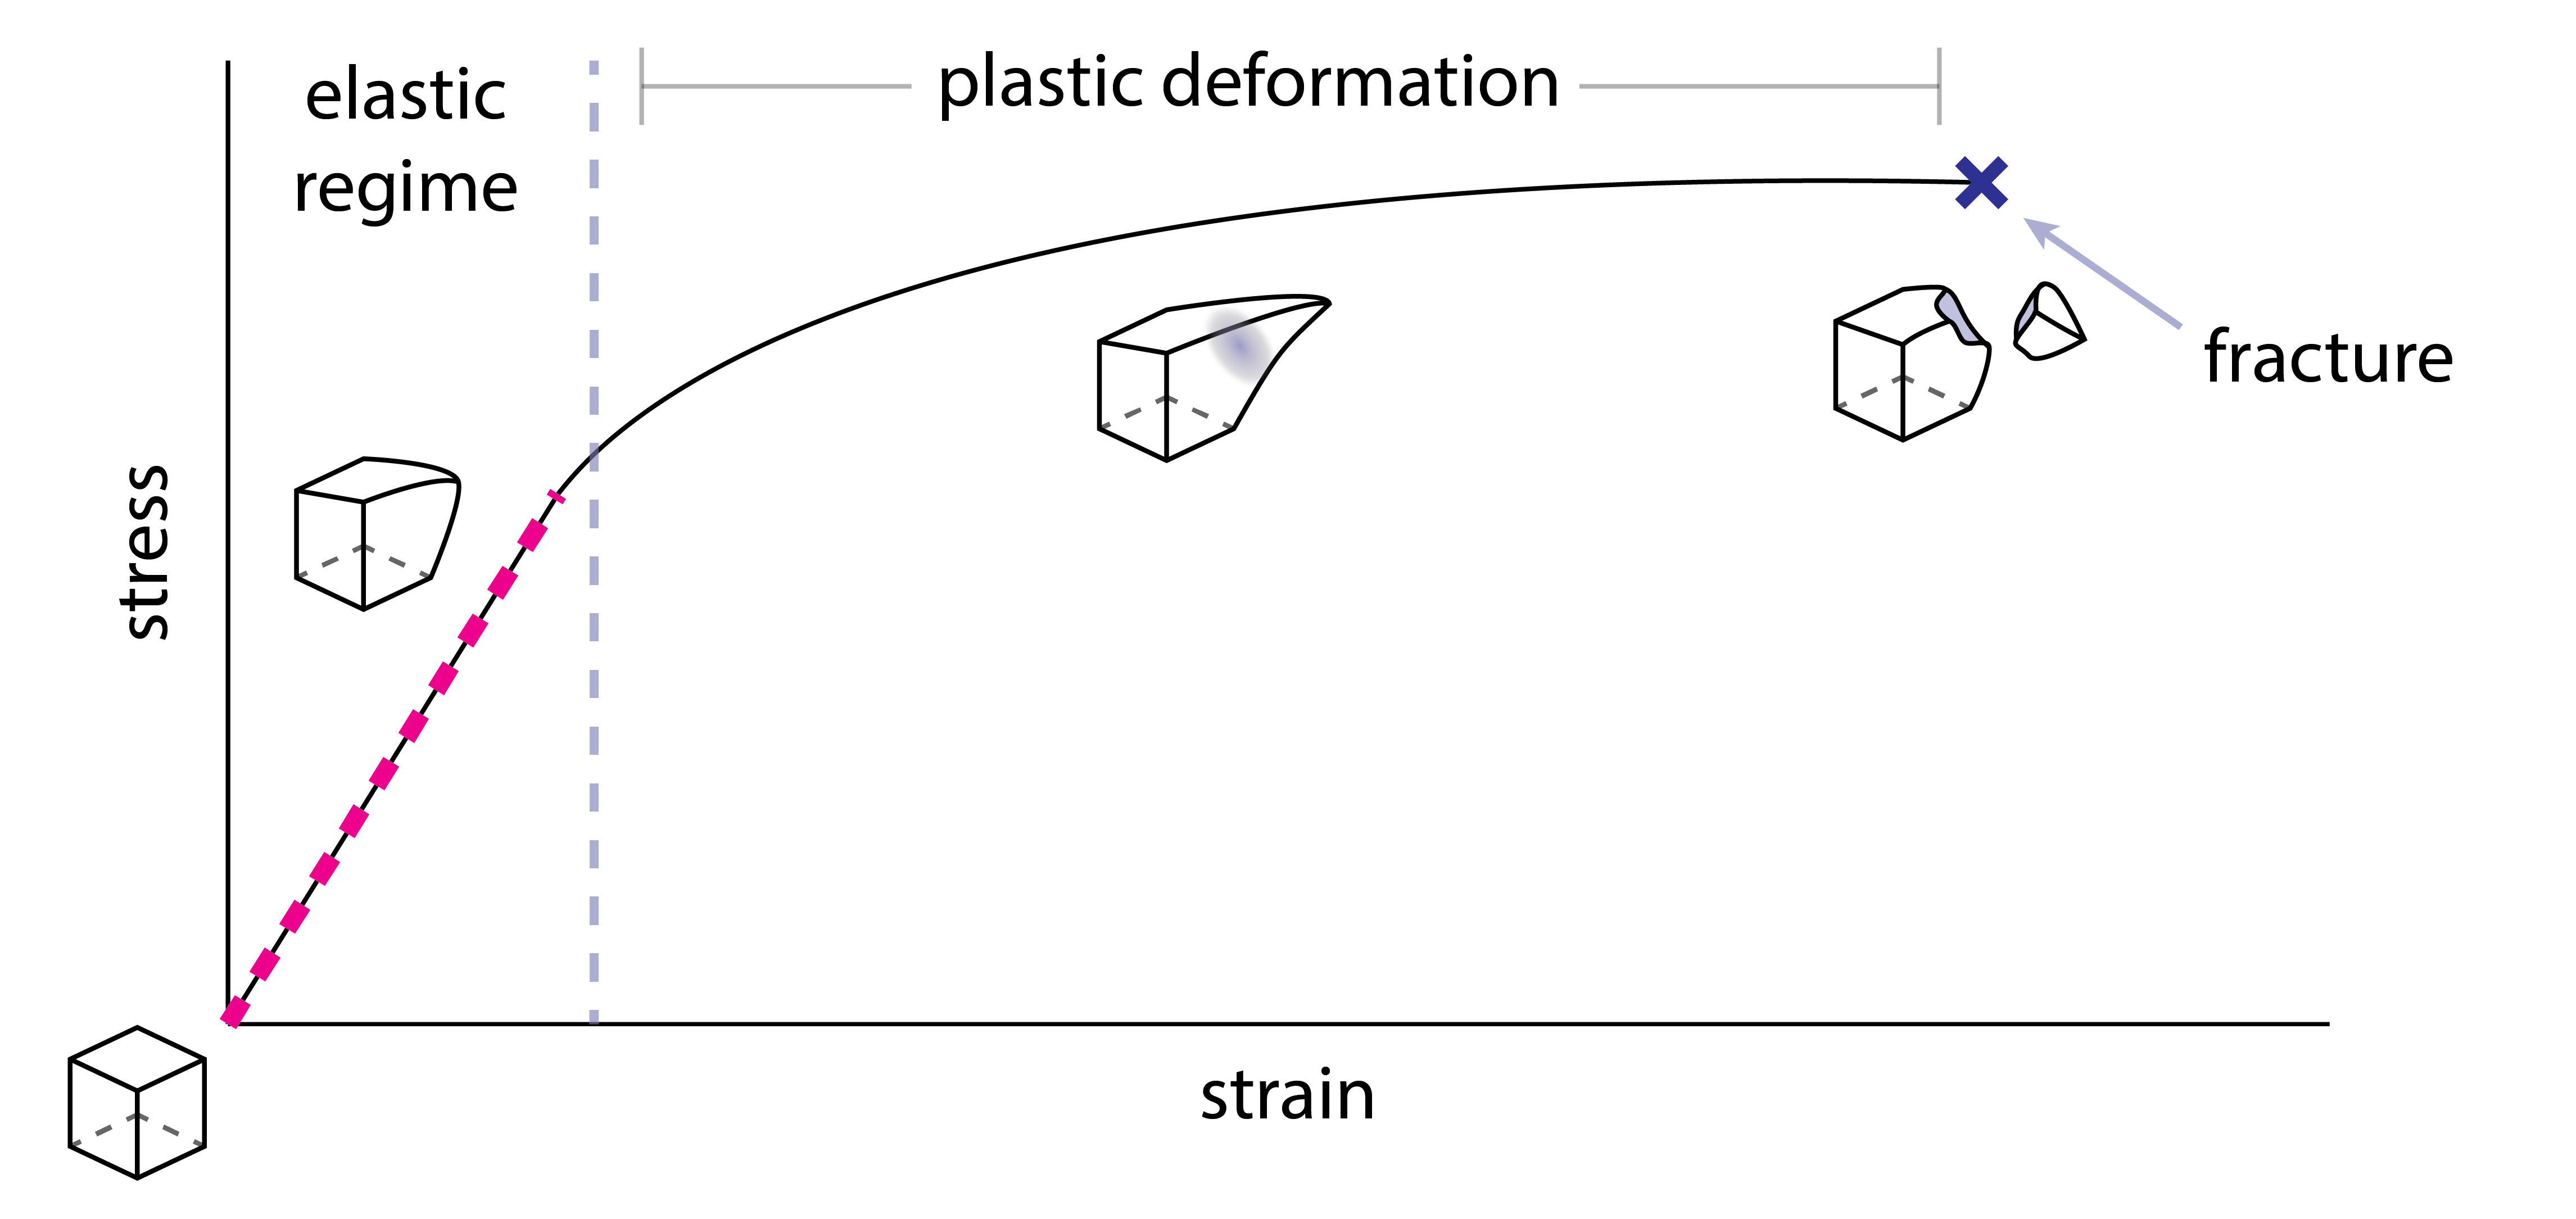
\includegraphics[width=\linewidth]{SolidRegimes.png}
  \caption{Stress/strain curves of materials reveal the linear elastic regime (pink), characterized by linear relationship between stress and strain.  Under larger stresses, materials enter non-linear elastic and plastic deformations, and eventually fracture.}
  \label{fig:SolidRegimes}
\end{figure}

The behavior of solids is typically characterized in terms of \textit{stress} and \textit{strain}.  Stress describes the internal and external forces acting on a material, measured as force per area in pascals (Pa) or N/m\textsuperscript{2}.  Strain describes the deformations of a material in response to stress, measured as a unit-less ratio of a length of deformation per unit of unstressed length.  Figure \ref{fig:SolidRegimes} shows an example of a typical stress/strain curve for a solid material.\\

Solids deform in an elastic regime until stresses acting on or within them become so large they result in irreversible, plastic deformations or fracture.  The modeling in this chapter will deal exclusively with \textit{linear} elastic deformations of solids.  This is the region of the stress/strain curve with constant slope, indicated by the pink dotted line in Figure \ref{fig:SolidRegimes}.  In this region, stress and strain have an approximately linear relationship to each other, in other words, materials obey Hooke's law:
\[F = kx\]

where F is a force, x is a displacement, and k is a measure of geometric stiffness.  We can rewrite Hooke's law in terms of stress ($\sigma$) and strain ($\epsilon$) as follows:
\begin{equation}\label{eq:stressstrainaxial}
\sigma_{axial} = E\epsilon_{axial} 
\end{equation}
\begin{equation}\label{eq:stressstrainshear}
\sigma_{shear} = G\epsilon_{shear} 
\end{equation}

where $E$ is the elastic modulus (also called "Young's modulus") and G is the shear modulus of a material.  As long as the forces acting on and within a solid are sufficiently low, we can assume that these linear elastic deformation models apply.\\

\begin{figure}
  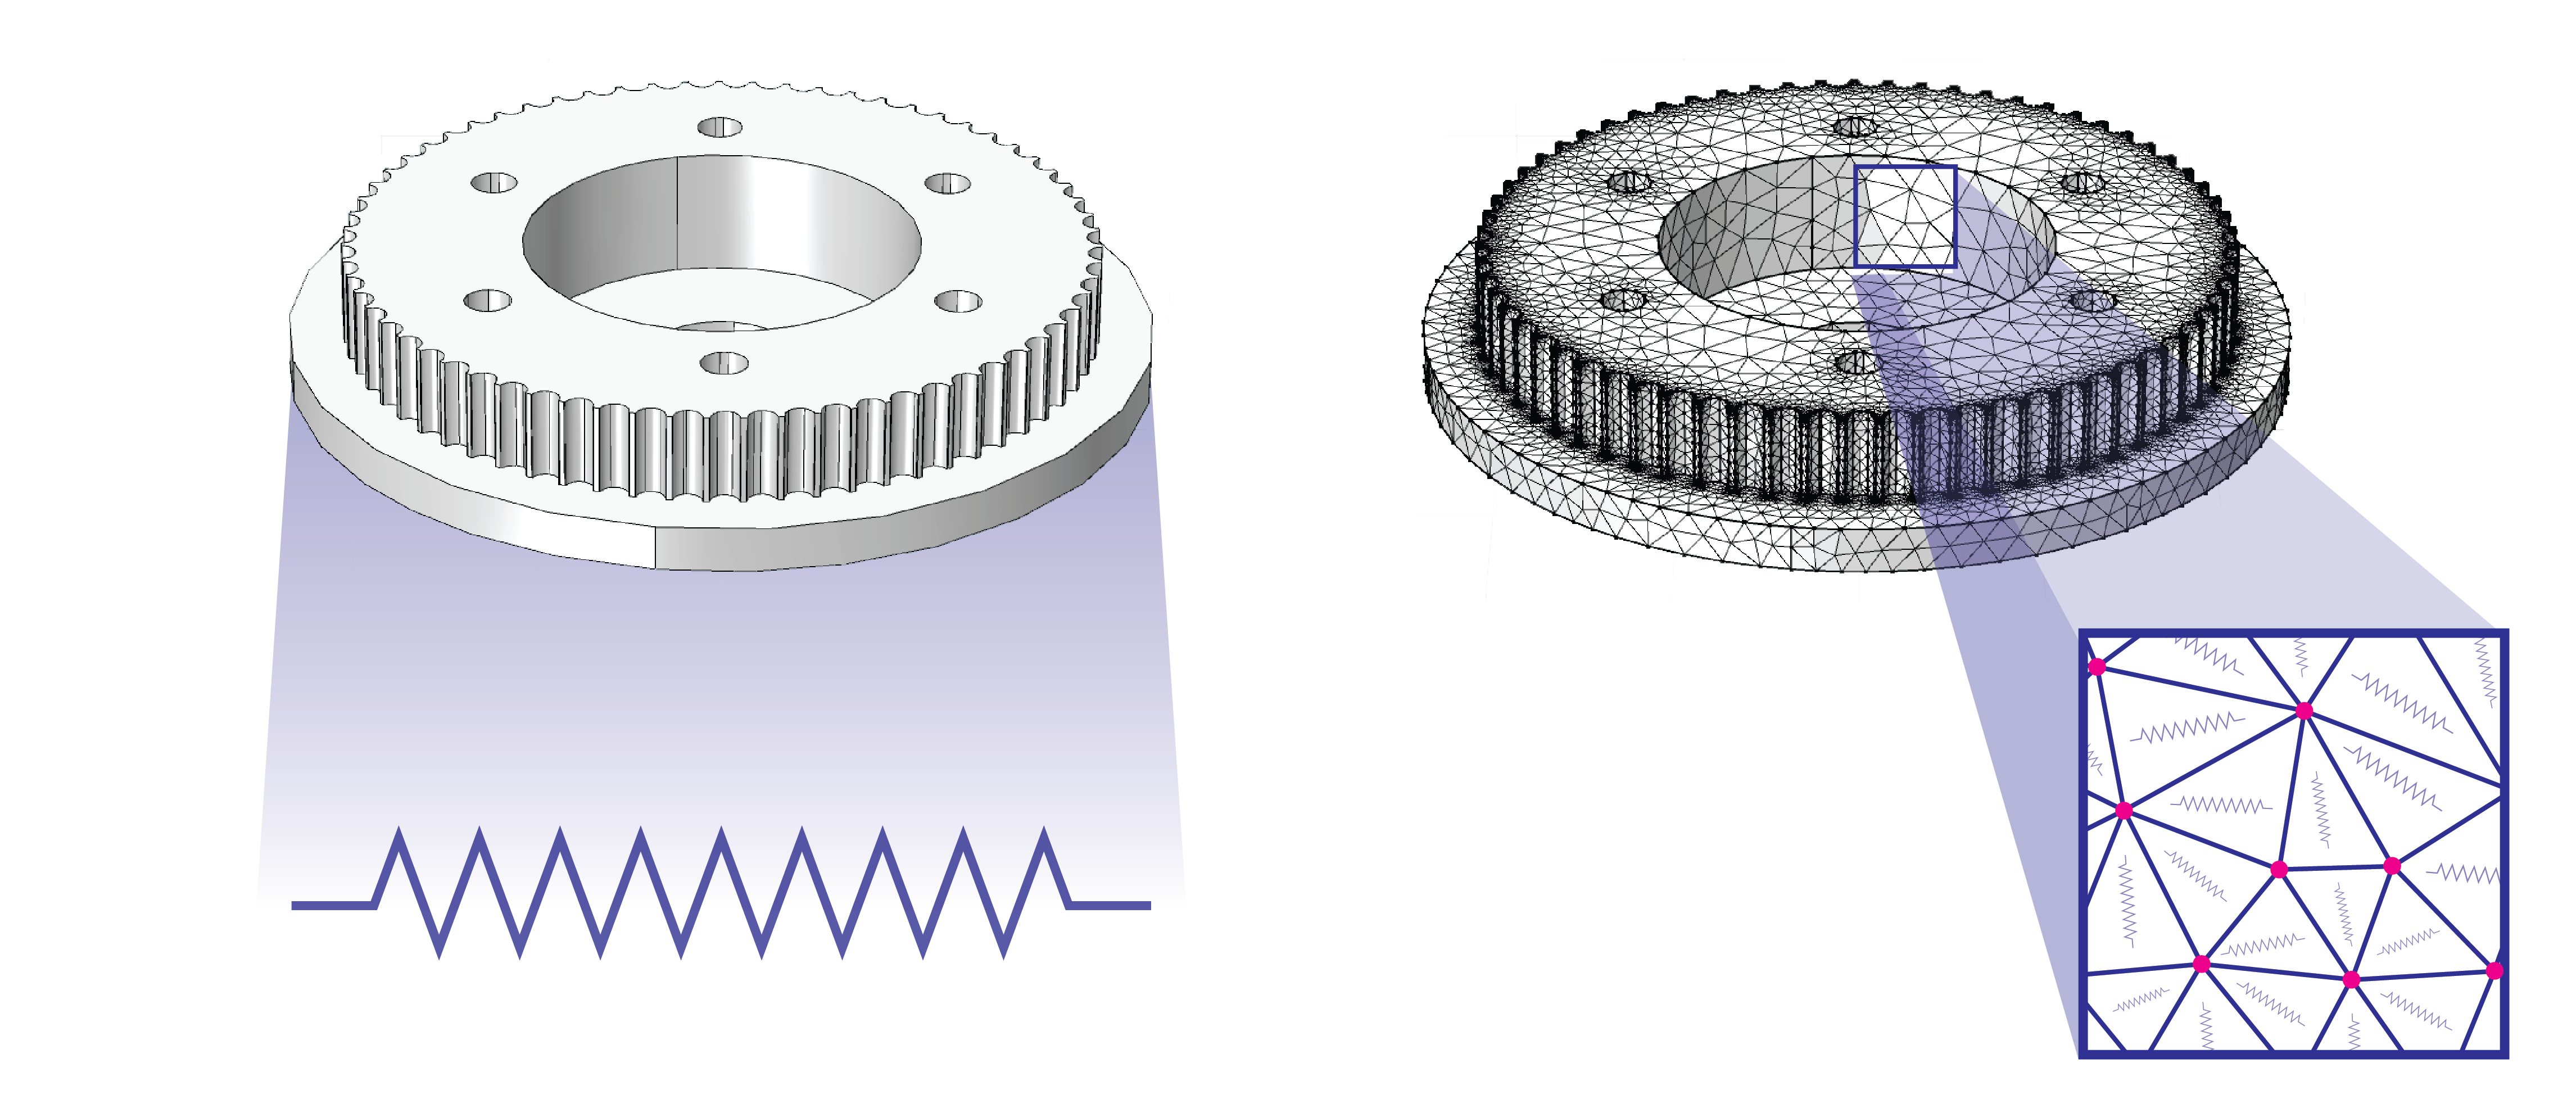
\includegraphics[width=\linewidth]{FEAexample.png}
  \caption{Two potential ways to model linear elastic deformations of a solid.  The strategy on the left treats the entire geometry as a Hookian spring, resulting in erroneous modeling of the solid's behavior.  The strategy on the left breaks up the solid into small regions which can individually be modeled with Hooke's law to a reasonable degree of accuracy.  The individual behaviors of the small regions are combined to synthesize a model of the global behavior of the entire geometry.  The method on the right summarizes the main idea behind traditional FEA.}
  \label{fig:FEAexample}
\end{figure}

So far we have discussed the ways that a solid's material properties, $E$ and $G$, affect its behavior, next we must consider its geometry.  Starting with Equations \ref{eq:stressstrainaxial} and  \ref{eq:stressstrainshear}, we could try modeling the deformations of a linear, elastic solid as a multi-dimentional Hookian spring with axial and shear stiffnesses $E$ and $G$.  Though this strategy could yield reasonable results for simple geometries and loading patterns, like a rubberband in pure tension, it is not accurate for more complex situations.  Instead, modern simulation techniques break up complex geometries into many simple, discrete regions whose individual behavior can be accurately modeled with Hooke's law (Figure \ref{fig:FEAexample}).  Combining the solutions to these discrete regions approximates the net behavior of the more complex geometry.  The process I've just described is typically referred to as \textit{Finite Element Analysis} (FEA).\\
%Finite Element Analysis (FEA) is essentially the process of applying Hooke's law to many small regions of a geometry and adding up their result.\\

\begin{figure}
  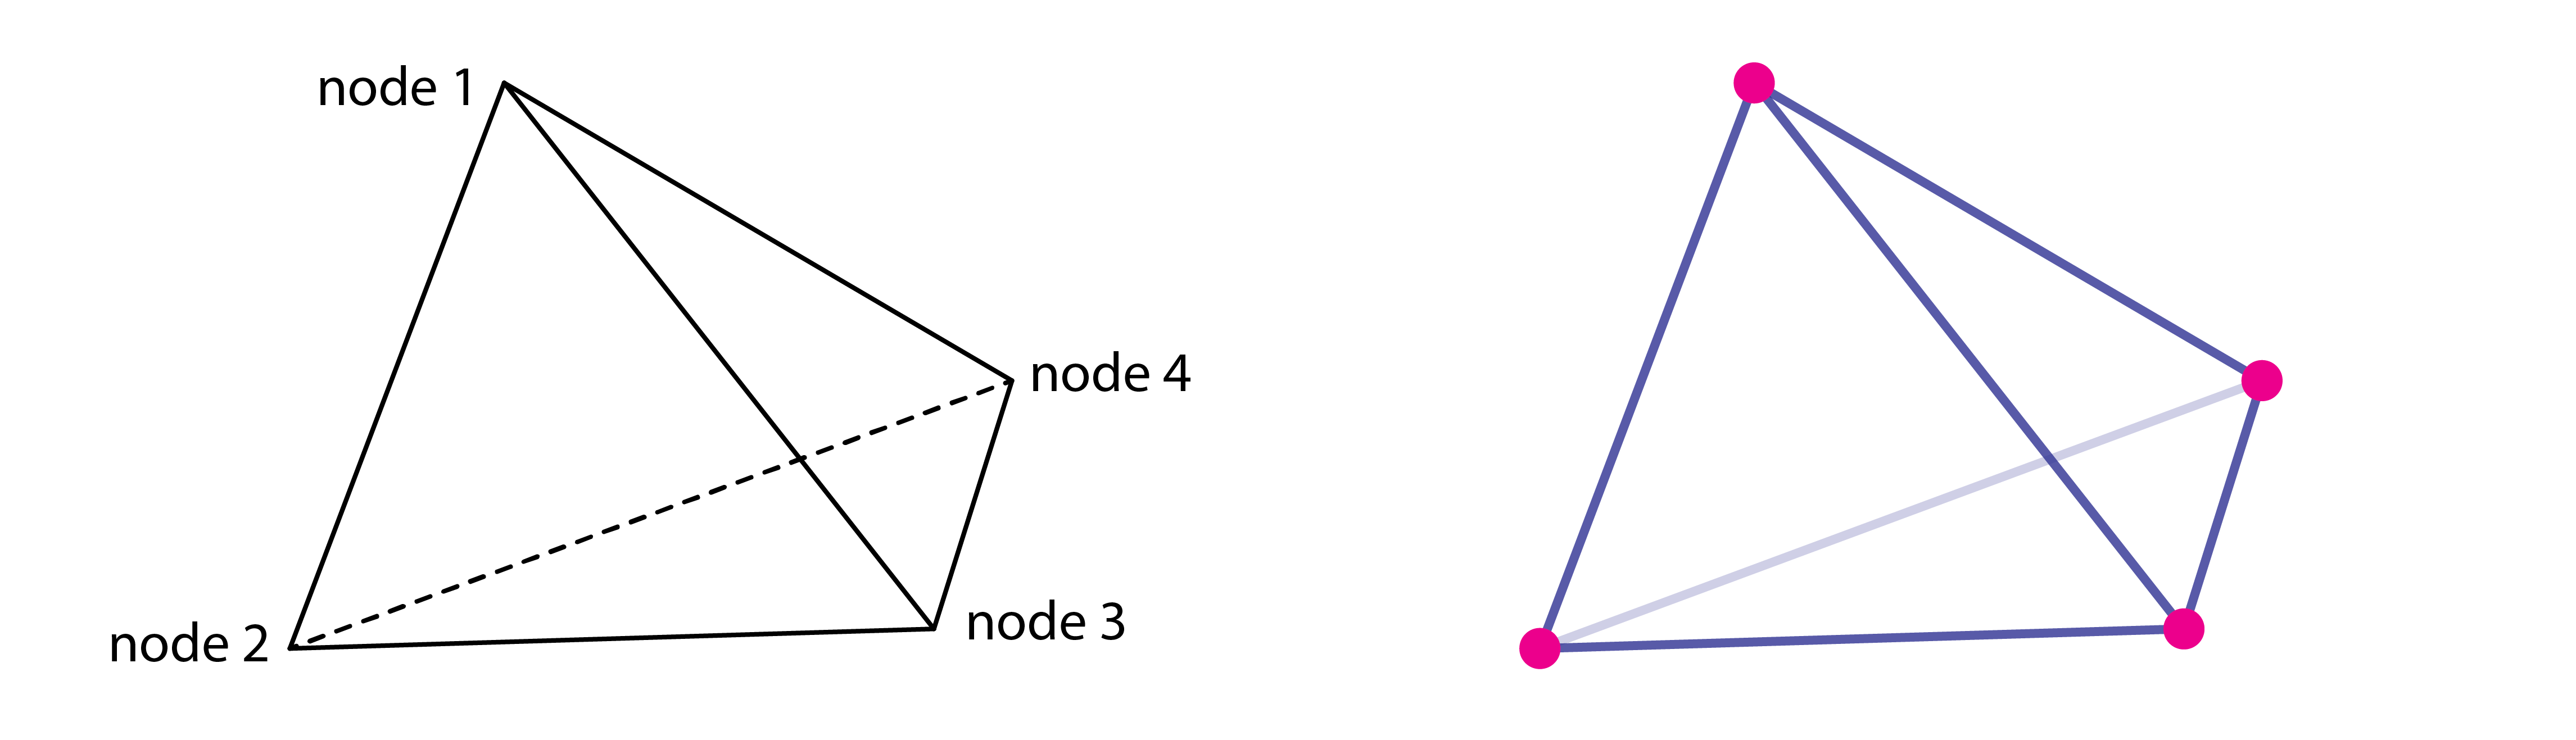
\includegraphics[width=\linewidth]{TetraElement.png}
  \caption{A tetrahedral element in 3D FEA.  The vertices of each element are called nodes.  In linear elastic solids, the relationships between forces (stress) and displacement (strain) of the nodes is described by variations on Hooke's law.  The springs indicated in the figure on the right are meant to illustrate the linear elastic (Hookian) relationship between nodes.  Typically, interactions between nodes are modeled with 6DOF linear elastic relationships as opposed to a 1DOF spring.}
  \label{fig:TetraElement}
\end{figure}

Now we can model the global deformations of a solid as the summation of deformations of many smaller, discrete volumes, or \textit{finite elements}.  In 3D, these elements might have any number of shapes, a common element shape is the tetrahedral illustrated in Figure \ref{fig:TetraElement}.  The vertices of each finite element are called nodes.  Nodes connect to other nodes through the edges of the elements to form a mesh.  No assumptions are made about the length of the edges of a finite element; in fact one of the main advantages of FEA is the ability to locally alter the resolution of the mesh in a particular region of interest.\\

\begin{figure}
  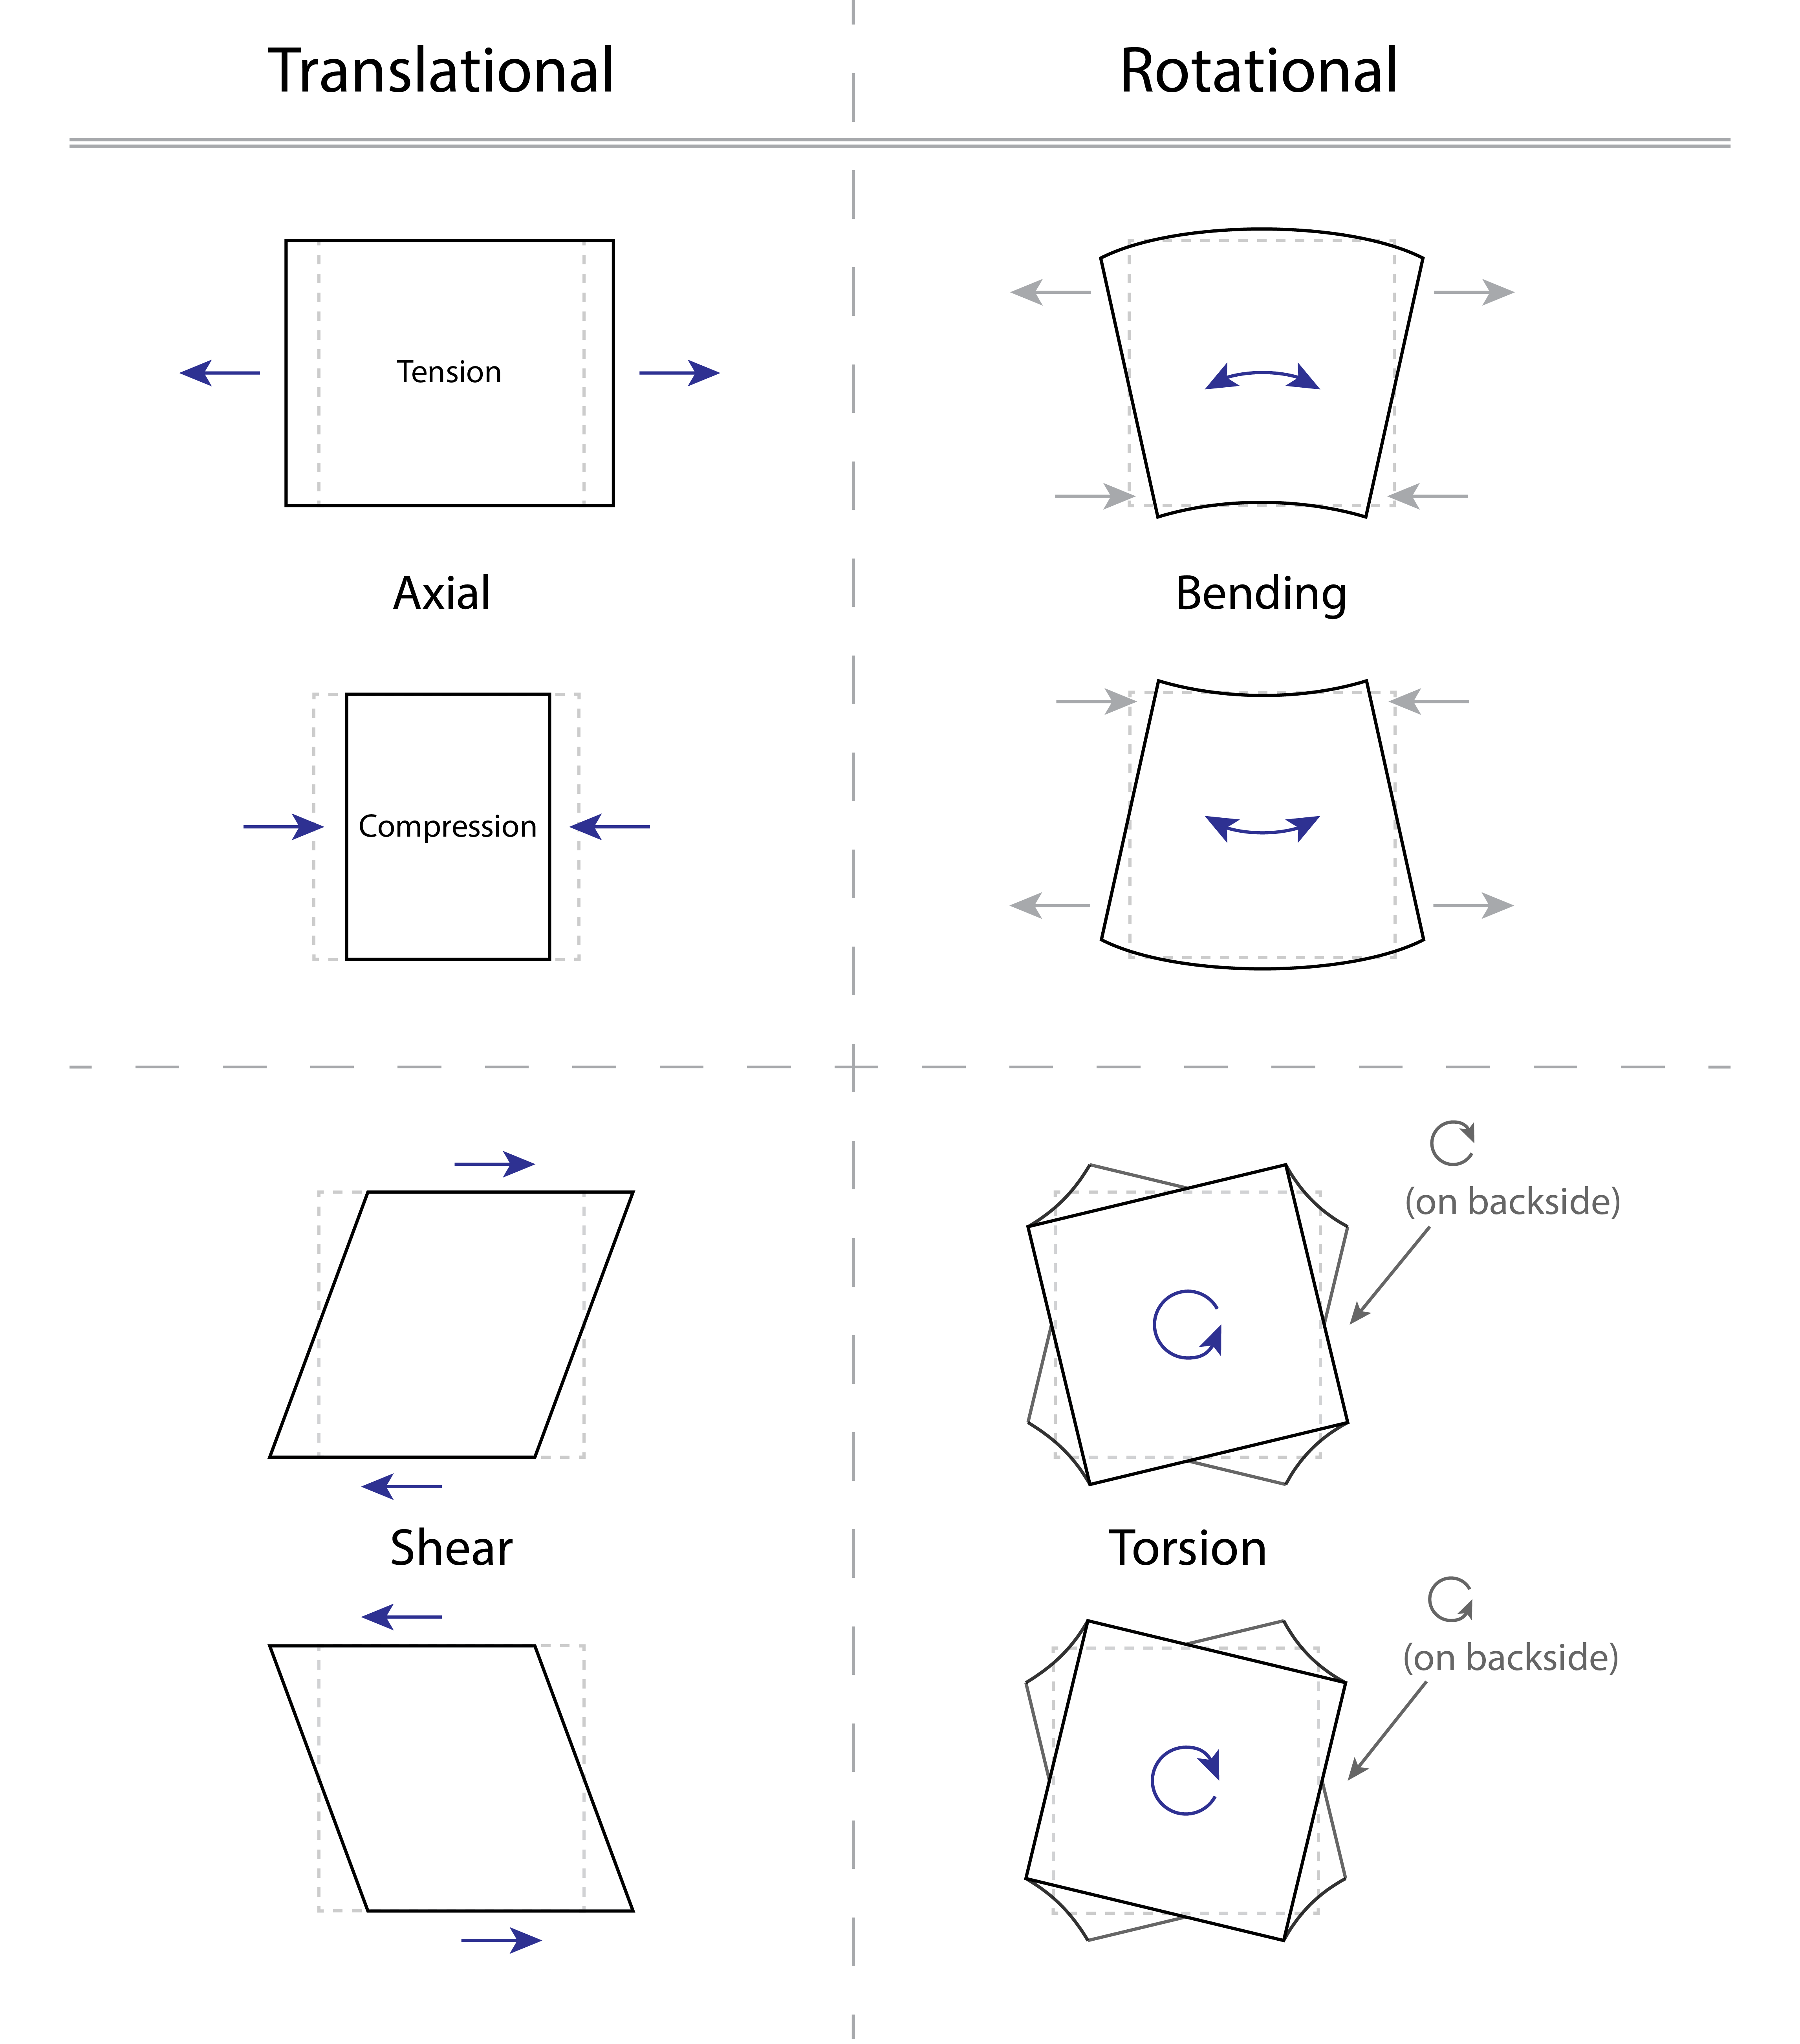
\includegraphics[width=\linewidth]{SolidMechanicsDOF.png}
  \caption{Deformations of a finite element under four types of applied forces.  In modeling assemblies of \textit{functional primitives}, these characteristic deformations are referred to as "internal degrees of freedom".  Within an assembly of cells, axial (compression and tension) and shear forces cause translational displacement and bending and torsional forces cause rotational displacement.}
  \label{fig:SolidMechanicsDOF}
\end{figure}

We must also consider that materials may respond differently to different types of forces.  Forces acting on finite elements fall into four categories: axial (tension and compression), shear, bending, and torsion.  Each type of applied force causes a characteristic deformation, illustrated in Figure \ref{fig:SolidMechanicsDOF}.  Applying multiple types of forces on a finite element will cause it to exhibit a combination of deformations.  We've seen how $E$ determines the behavior of a material in response to axial stress and $G$ for shear stress in Equations \ref{eq:stressstrainaxial} and  \ref{eq:stressstrainshear}.  Using information about the geometry of an element, we can derive equations for bending and torsional response in terms of torque ($T$) and angular displacement ($\theta$):
\begin{equation}\label{eq:stressstrainbending}
T_{bending} = \dfrac{EI}{l}\theta_{bending}\\[10pt]
\end{equation}
\begin{equation}\label{eq:stressstraintorsion}
T_{torsion} = \dfrac{GJ}{l}\theta_{torsion} 
\end{equation}

where I and J are area moment of inertias (a measure of the distribution of material in a cross section - convention uses $J$ for torsional cross section and $I$ for bending, but they are calculated the same way) and $l$ is the length of the element in the relevant direction.\\

Equations \ref{eq:stressstrainaxial}, \ref{eq:stressstrainshear}, \ref{eq:stressstrainbending}, and \ref{eq:stressstraintorsion} work nicely for homogenous materials, but don't address situations where a material's response depends on the direction of the applied stress.  A material is isotropic if it responds the same to a stress in any orientation.  Materials comprised of oriented fibers or other internal structure typically display anisotropic behaviors.  Most FEA methods and tools assume finite elements are isotropic.

\section{Modeling Setup}

\begin{figure}
  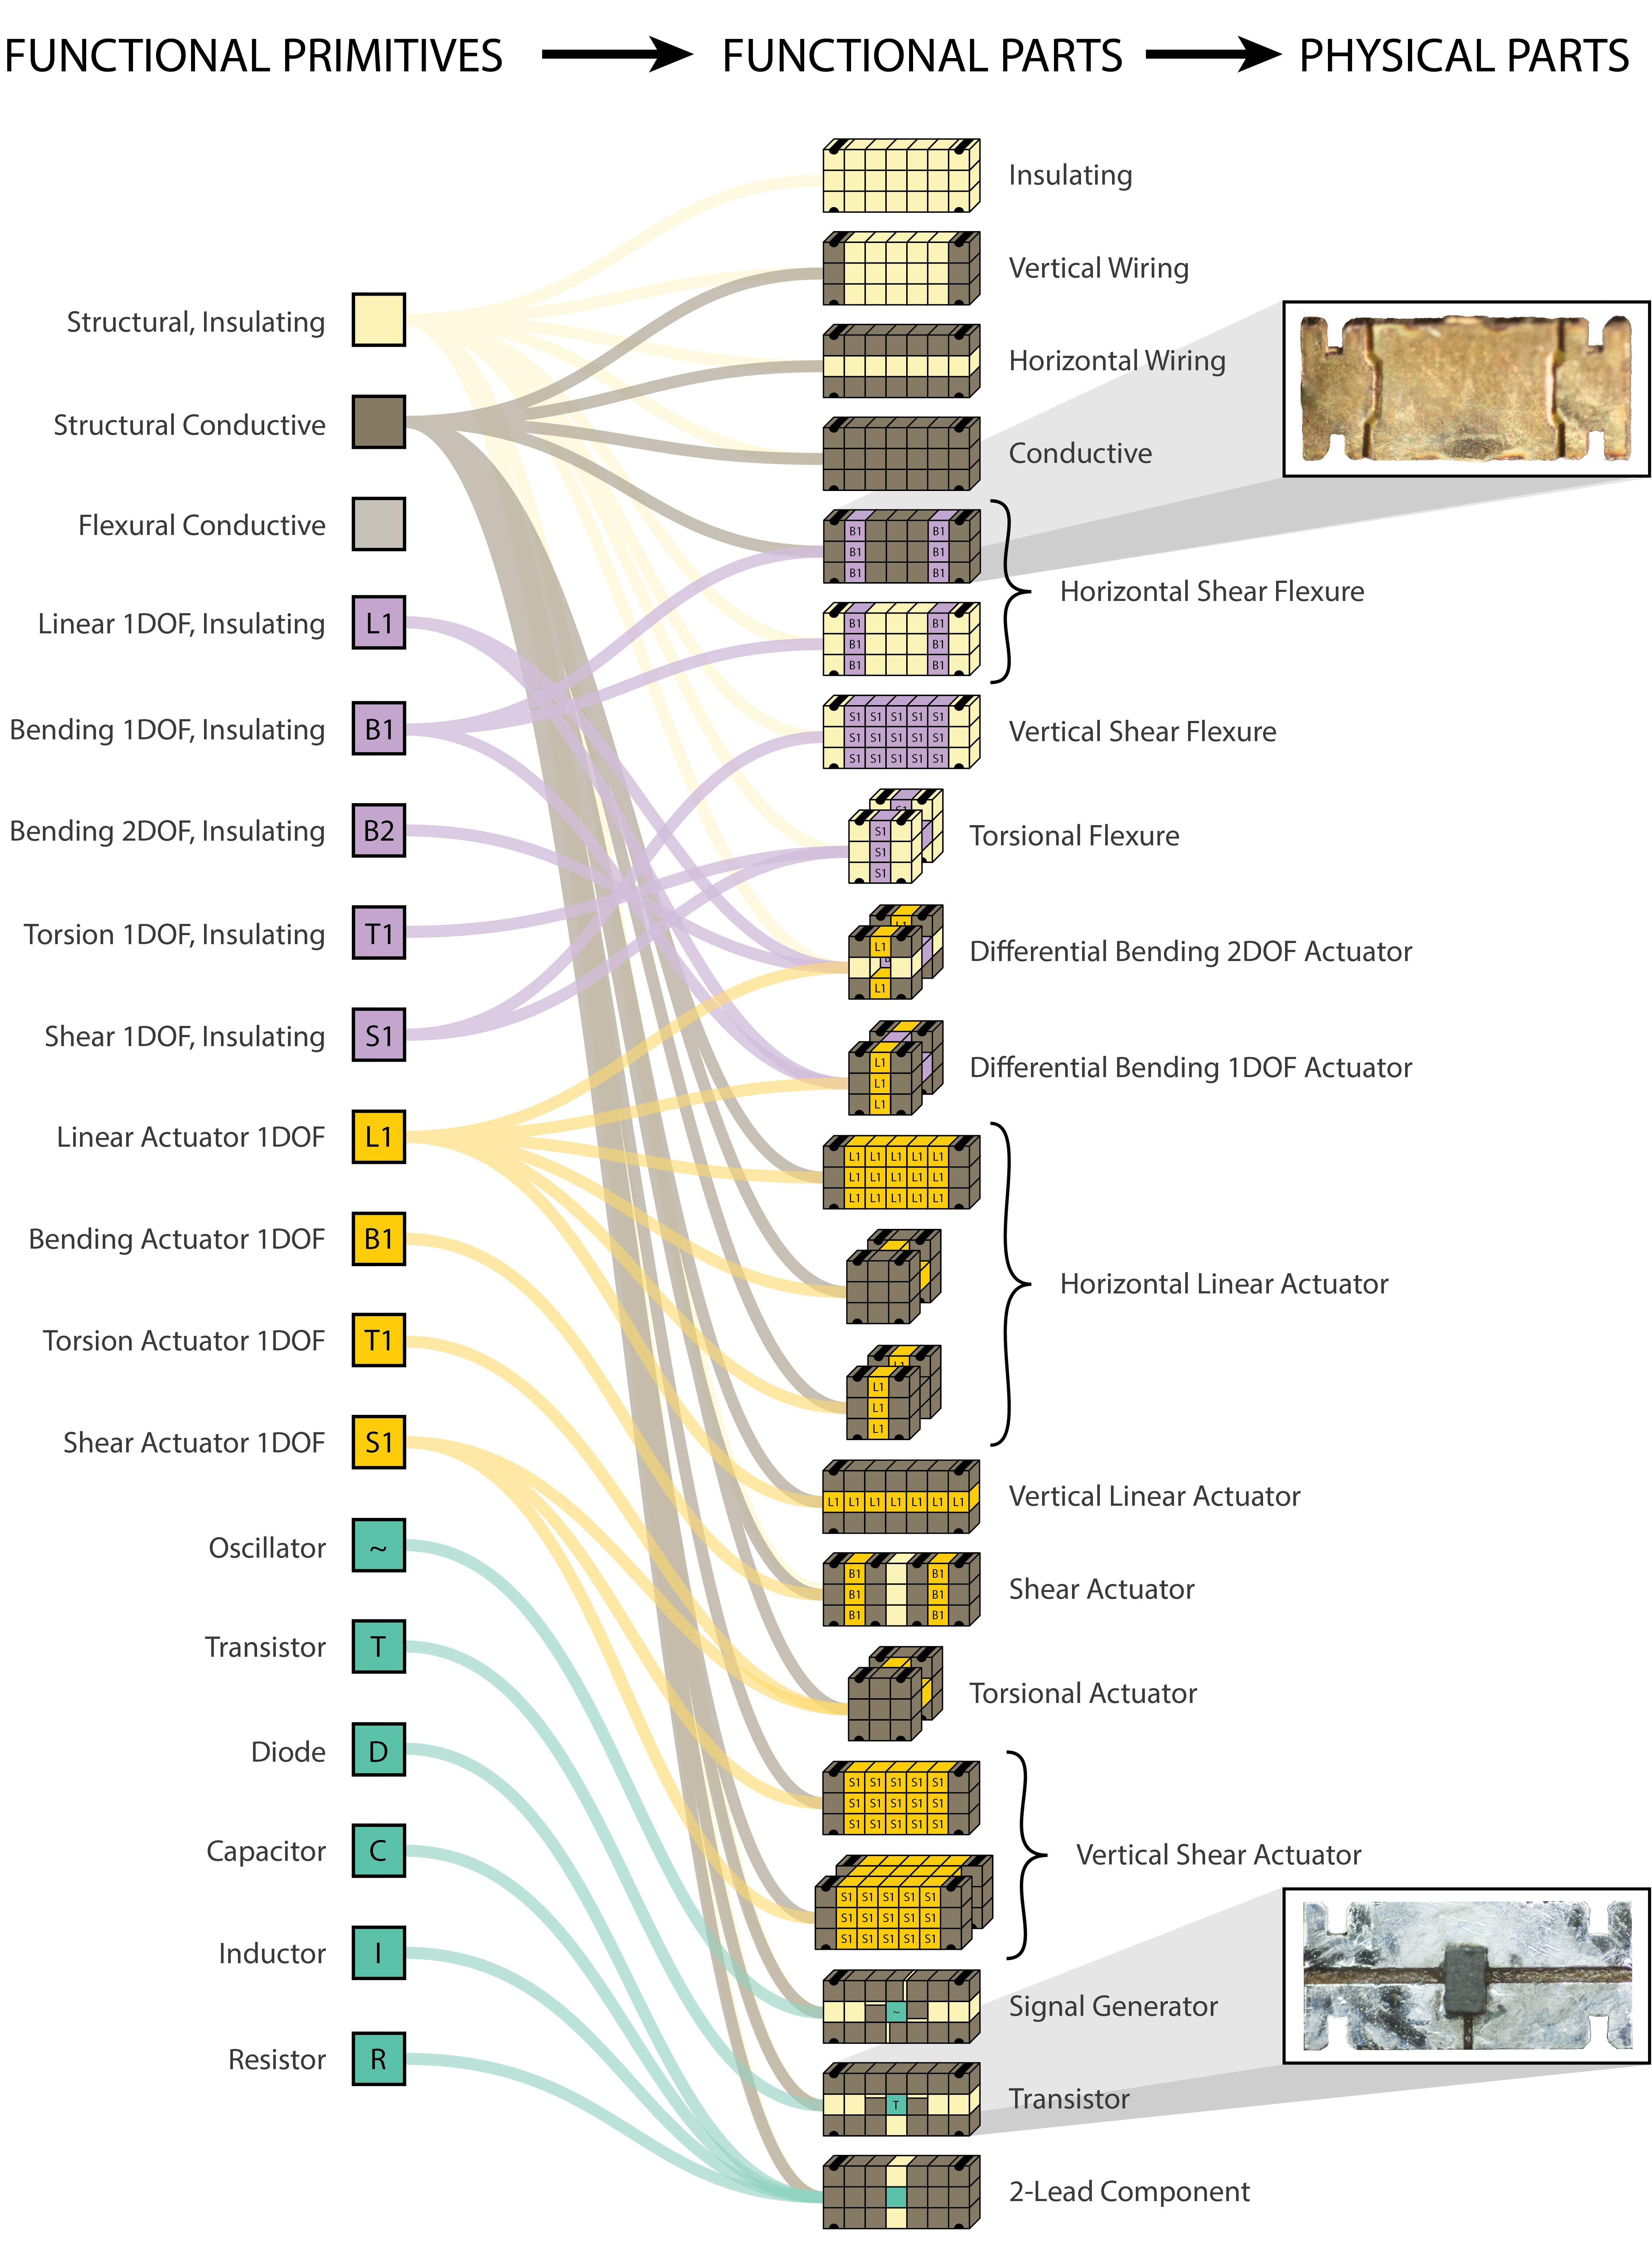
\includegraphics[width=\linewidth]{FunctionPrimitivesPartsWPic.png}
  \caption{Illustration of various functional parts, showing their decomposition into functional primitives.  Simulation of functional parts occurs at the granularity of functional primitives.  Fabricated transistor and shear flexure shown alongside its virtual representation.  \textit{Image Credit: (photos of physical parts) Will Langford 2016}}
  \label{fig:FunctionPrimitivesPartsWPic}
\end{figure}

Simulation of an assembly of \textit{functional parts} happens at the granularity of identically-sized \textit{functional primitives}, which I'll call "cells" for the remainder of this chapter.  Functional parts, their decomposition into functional primitives, and the physical parts being modeled are illustrated in Figure \ref{fig:FunctionPrimitivesPartsWPic}.  The number of functional primitives shown in each functional part is meant only as an illustration for now; the exact aspect ratio and joining strategy between functional parts is still in development.  Once these parameters have been settled, the model can be adjusted to fit the parts simply by varying the scale and aspect ratio of the cubic lattice.\\

In the next sections, I'll demonstrate how to extend the ideas from FEA to model the dynamic behavior of multimaterial assemblies of identically-sized, anisotropic cells.  The primary motivations for this work are listed below:\\

\textbf{Exploit discretization of the physical system:} Functional parts are assembled on a regular, cubic lattice.  Rather than using an arbitrary mesh (as is the case in Figure \ref{fig:FEAexample}), we can decompose assemblies of parts into identically-shaped cells on a cubic lattice for simulation.  This will increase computational efficiency and should result in better agreement with empirical data \cite{Calisch2014}.\\

\textbf{Non-linear treatment of angular displacements:} Some flexures and actuators may exhibit large angular deformations that must be handled using non-linear (spherical) techniques.  Most FEA packages rely on small angle approximations to handle small angular deformations and costly remeshing to handle larger deformations without introducing error.\\

\textbf{Model multimaterial interactions:} Cells in this simulation are made from several material types which may be patterned together in close proximity.  In this model, dissimilar material properties may be combined and applied to interactions between different cell types.\\

\textbf{Anisotropy:} Cells may exhibit both isotropic and anisotropic behaviors.  To handle anisotropy, cell materials are parameterized by 15 stiffness and damping constants rather than just $E$ and $G$.\\

\textbf{Electronics and actuation:} Cells at the function-level are defined not only by their mechanical properties, but also by their ability to transmit electronic signals from one face to another, and their active properties in response to a signal.  This model provides a computationally efficient way to integrate electronic effects with mechanical simulation. \\

\begin{figure}
  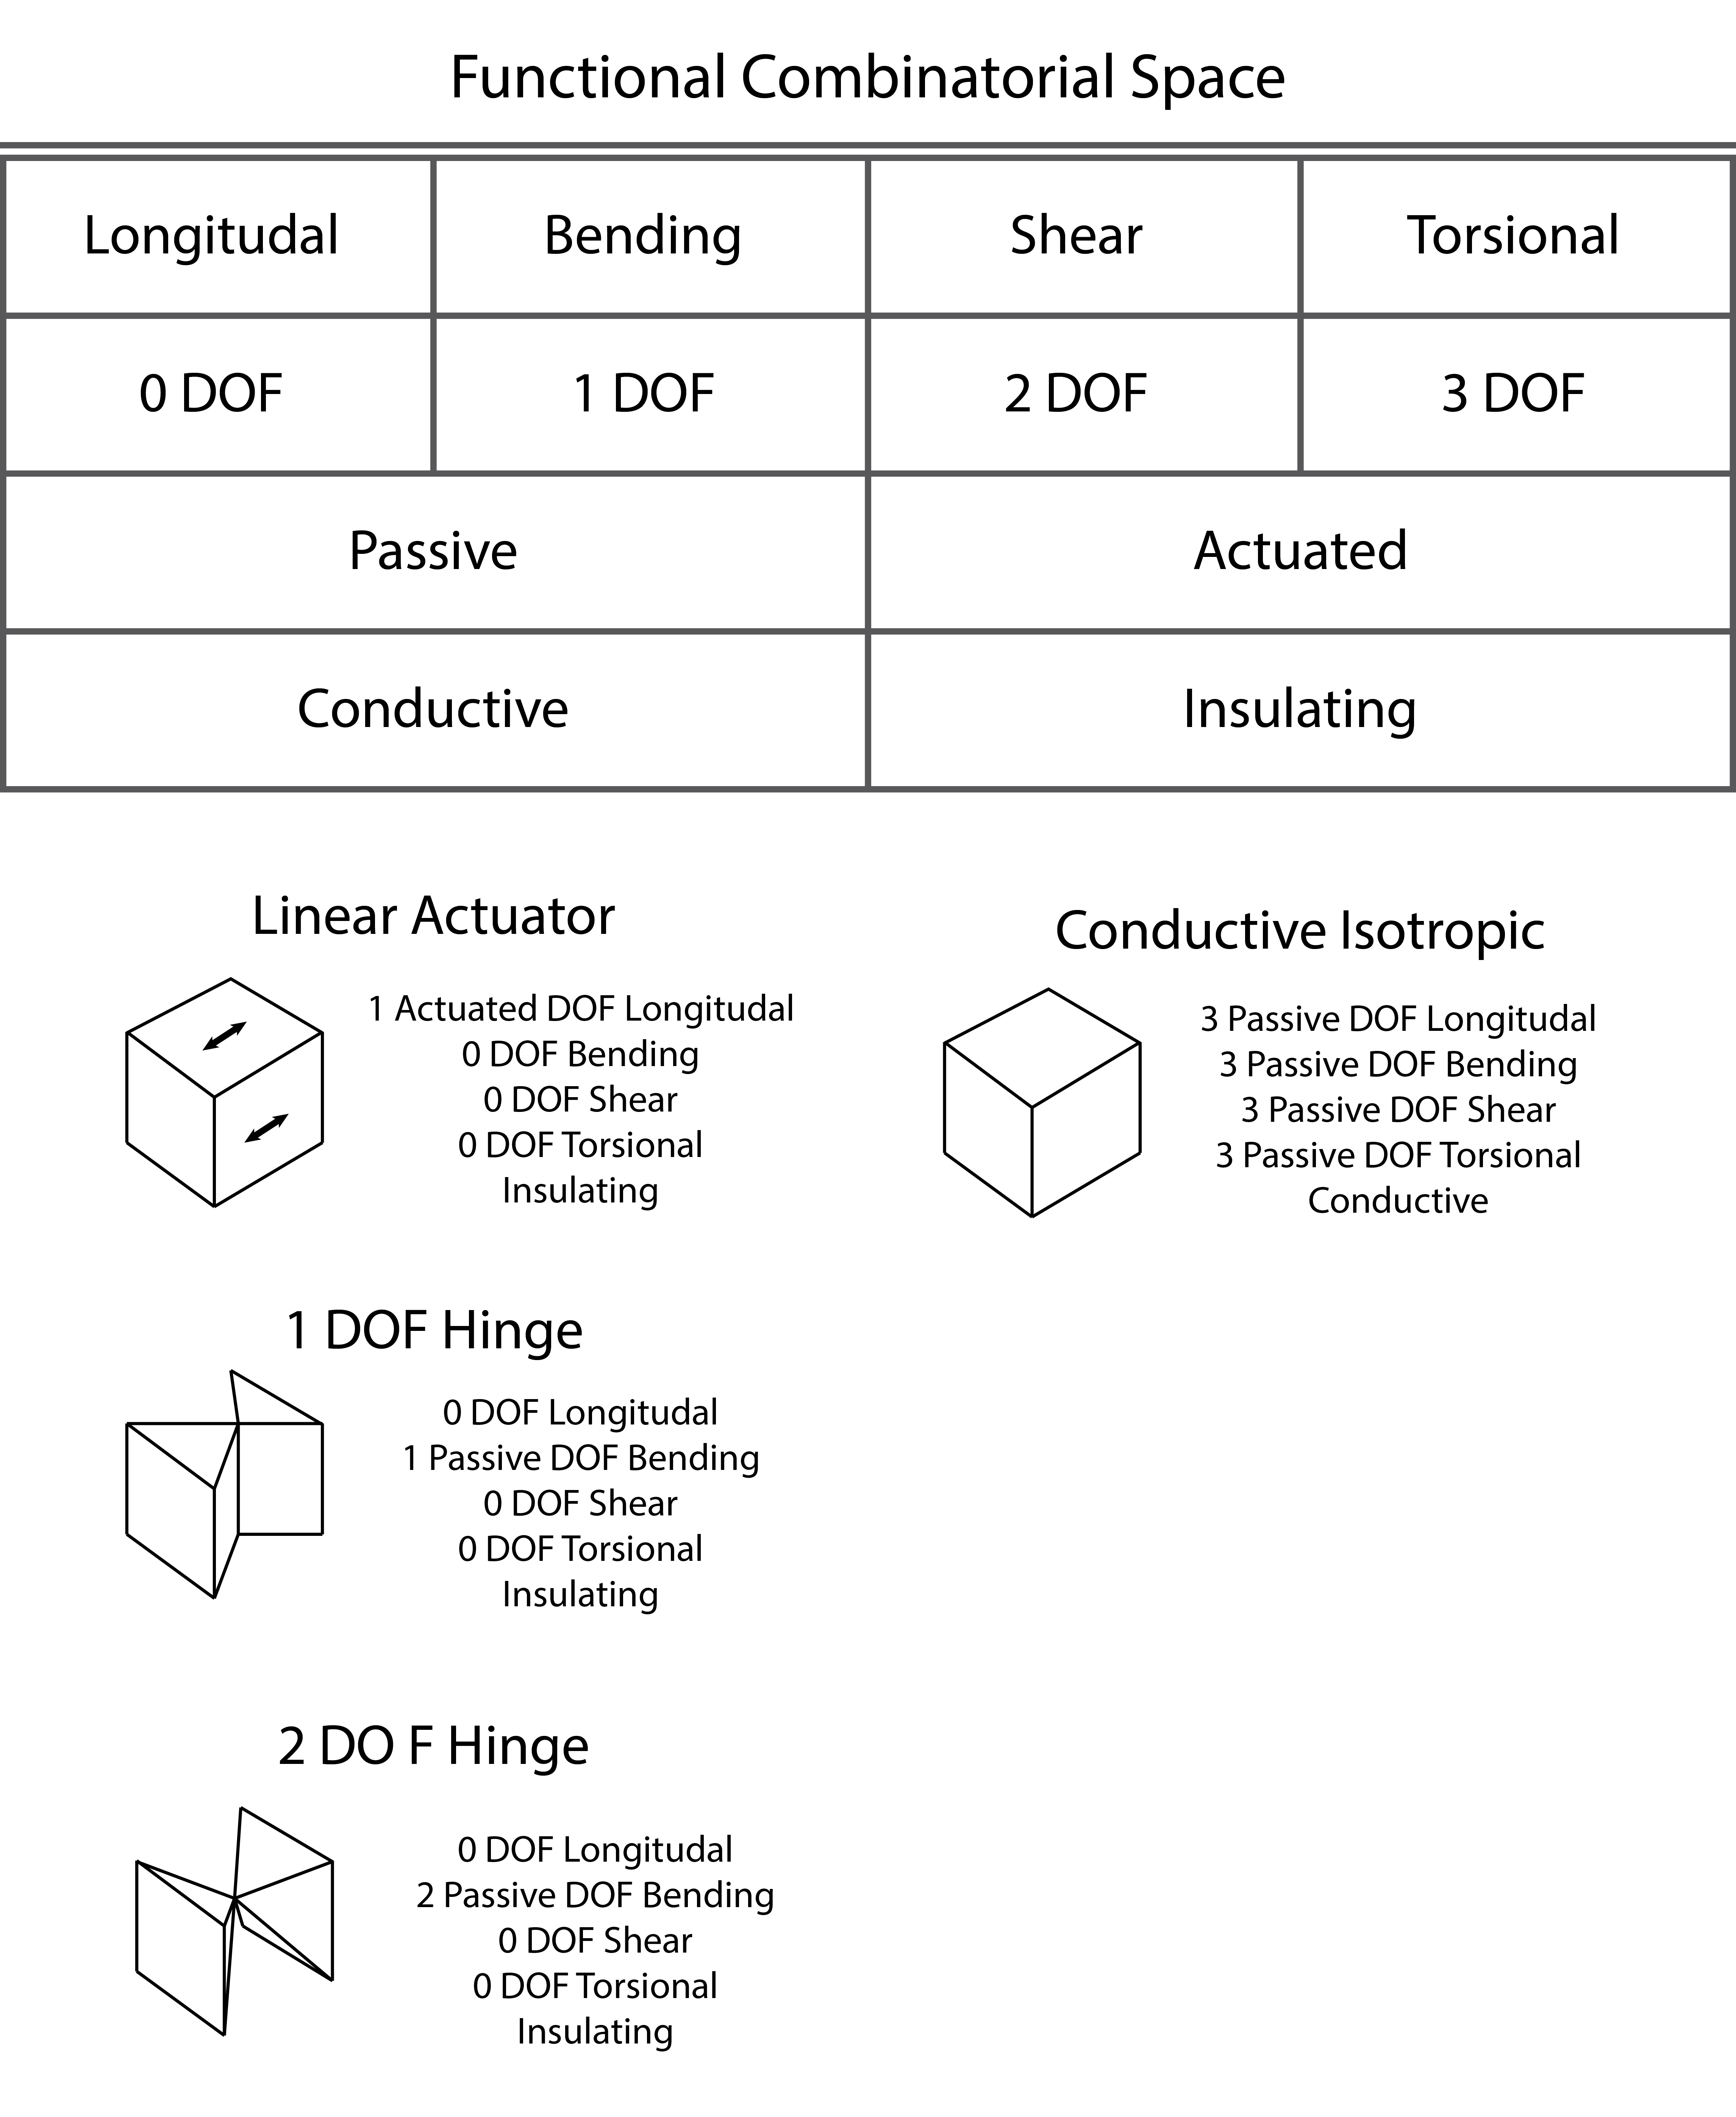
\includegraphics[width=\linewidth]{CombinatoricsOfFunctions.png}
  \caption{Combinatorial space of functional primitives with six examples explicitly described in terms of their electronic and mechanical properties.  Note - any individual degree of freedom within a cell falls on the spectrum described in Figure \ref{fig:BendingStiffnessContinuoum}.  A cell is described at a high level as having a particular degree of freedom if its corresponding stiffness in that dimension is sufficiently flexible to allow for significant deformation under applied load.  There are no infinitely stiff or fully unconstrained degrees of freedom in this system.}
  \label{fig:CombinatoricsOfFunctions}
\end{figure}

 The combinatorial space of mechanical, electronic, and actuated cell types is described in Figure \ref{fig:CombinatoricsOfFunctions}.  A selection of these cell types are included in Figure \ref{fig:FunctionPrimitivesPartsWPic} and have been implemented in simulation.  When describing mechanical behavior of a particular cell type, I'll refer to its four deformation modes (Figure \ref{fig:SolidMechanicsDOF}) as "internal degrees of freedom" (DOF).  For example, a 1-DOF bending cell will have large deformations in bending along one axis, but relatively small deformations in response to other types of applied forces.  Section \ref{sec:electronicSim} describes the process of electronic simulation in more detail, the remainder of this chapter will focus on the passive and active mechanical simulation of functional primitive cells.

\section{Spring-Damper Characteristics}

The geometric stiffness of a structure relates the bulk properties of a material to its 3d geometry.  For example, an I-beam has a higher geometric bending stiffness than an equal length rectangular bar made from the same amount of the same material.  Unless otherwise noted, "stiffness" in this analysis refers to geometric stiffness.\\

Stiffness and damping are used to characterize the response of cell's internal degrees of freedom to applied external forces.  Stiffness has the units N/m and damping N$\cdot$s/m.  In three dimensions, each cell's passive mechanical properties are parameterized by 15 stiffness and damping constants:

\[ k  = \begin{cases}
\enspace k_{axial_x}\\
\enspace k_{axial_y}\\
\enspace k_{axial_z}\\
\\
\enspace k_{shear_{xy}}\\
\enspace k_{shear_{xz}}\\
\enspace k_{shear_{yx}}\\
\enspace k_{shear_{yz}}\\
\enspace k_{shear_{zx}}\\
\enspace k_{shear_{zy}}\\
\\
\enspace k_{bending_x}\\
\enspace k_{bending_y}\\
\enspace k_{bending_z}\\
\\
\enspace k_{torsional_x}\\
\enspace k_{torsional_y}\\
\enspace k_{torsional_z}
 \end{cases}
 \qquad\qquad
 d  = \begin{cases}
\enspace d_{axial_x}\\
\enspace d_{axial_y}\\
\enspace d_{axial_z}\\
\\
\enspace d_{shear_{xy}}\\
\enspace d_{shear_{xz}}\\
\enspace d_{shear_{yx}}\\
\enspace d_{shear_{yz}}\\
\enspace d_{shear_{zx}}\\
\enspace d_{shear_{zy}}\\
\\
\enspace d_{bending_x}\\
\enspace d_{bending_y}\\
\enspace d_{bending_z}\\
\\
\enspace d_{torsional_x}\\
\enspace d_{torsional_y}\\
\enspace d_{torsional_z}
 \end{cases}  \]
\\

$k_{shear}$ and $d_{shear}$ are broken out into six parameters of the form $shear_{nm}$ because the shear response depends both on the direction of shear displacement between two cells ($m$) and on the axis along which the cells are connected ($n$).  The $shear_{nm}$ notion used above is described graphically in in Figure \ref{fig:ShearDOFs}.\\

\begin{figure}
  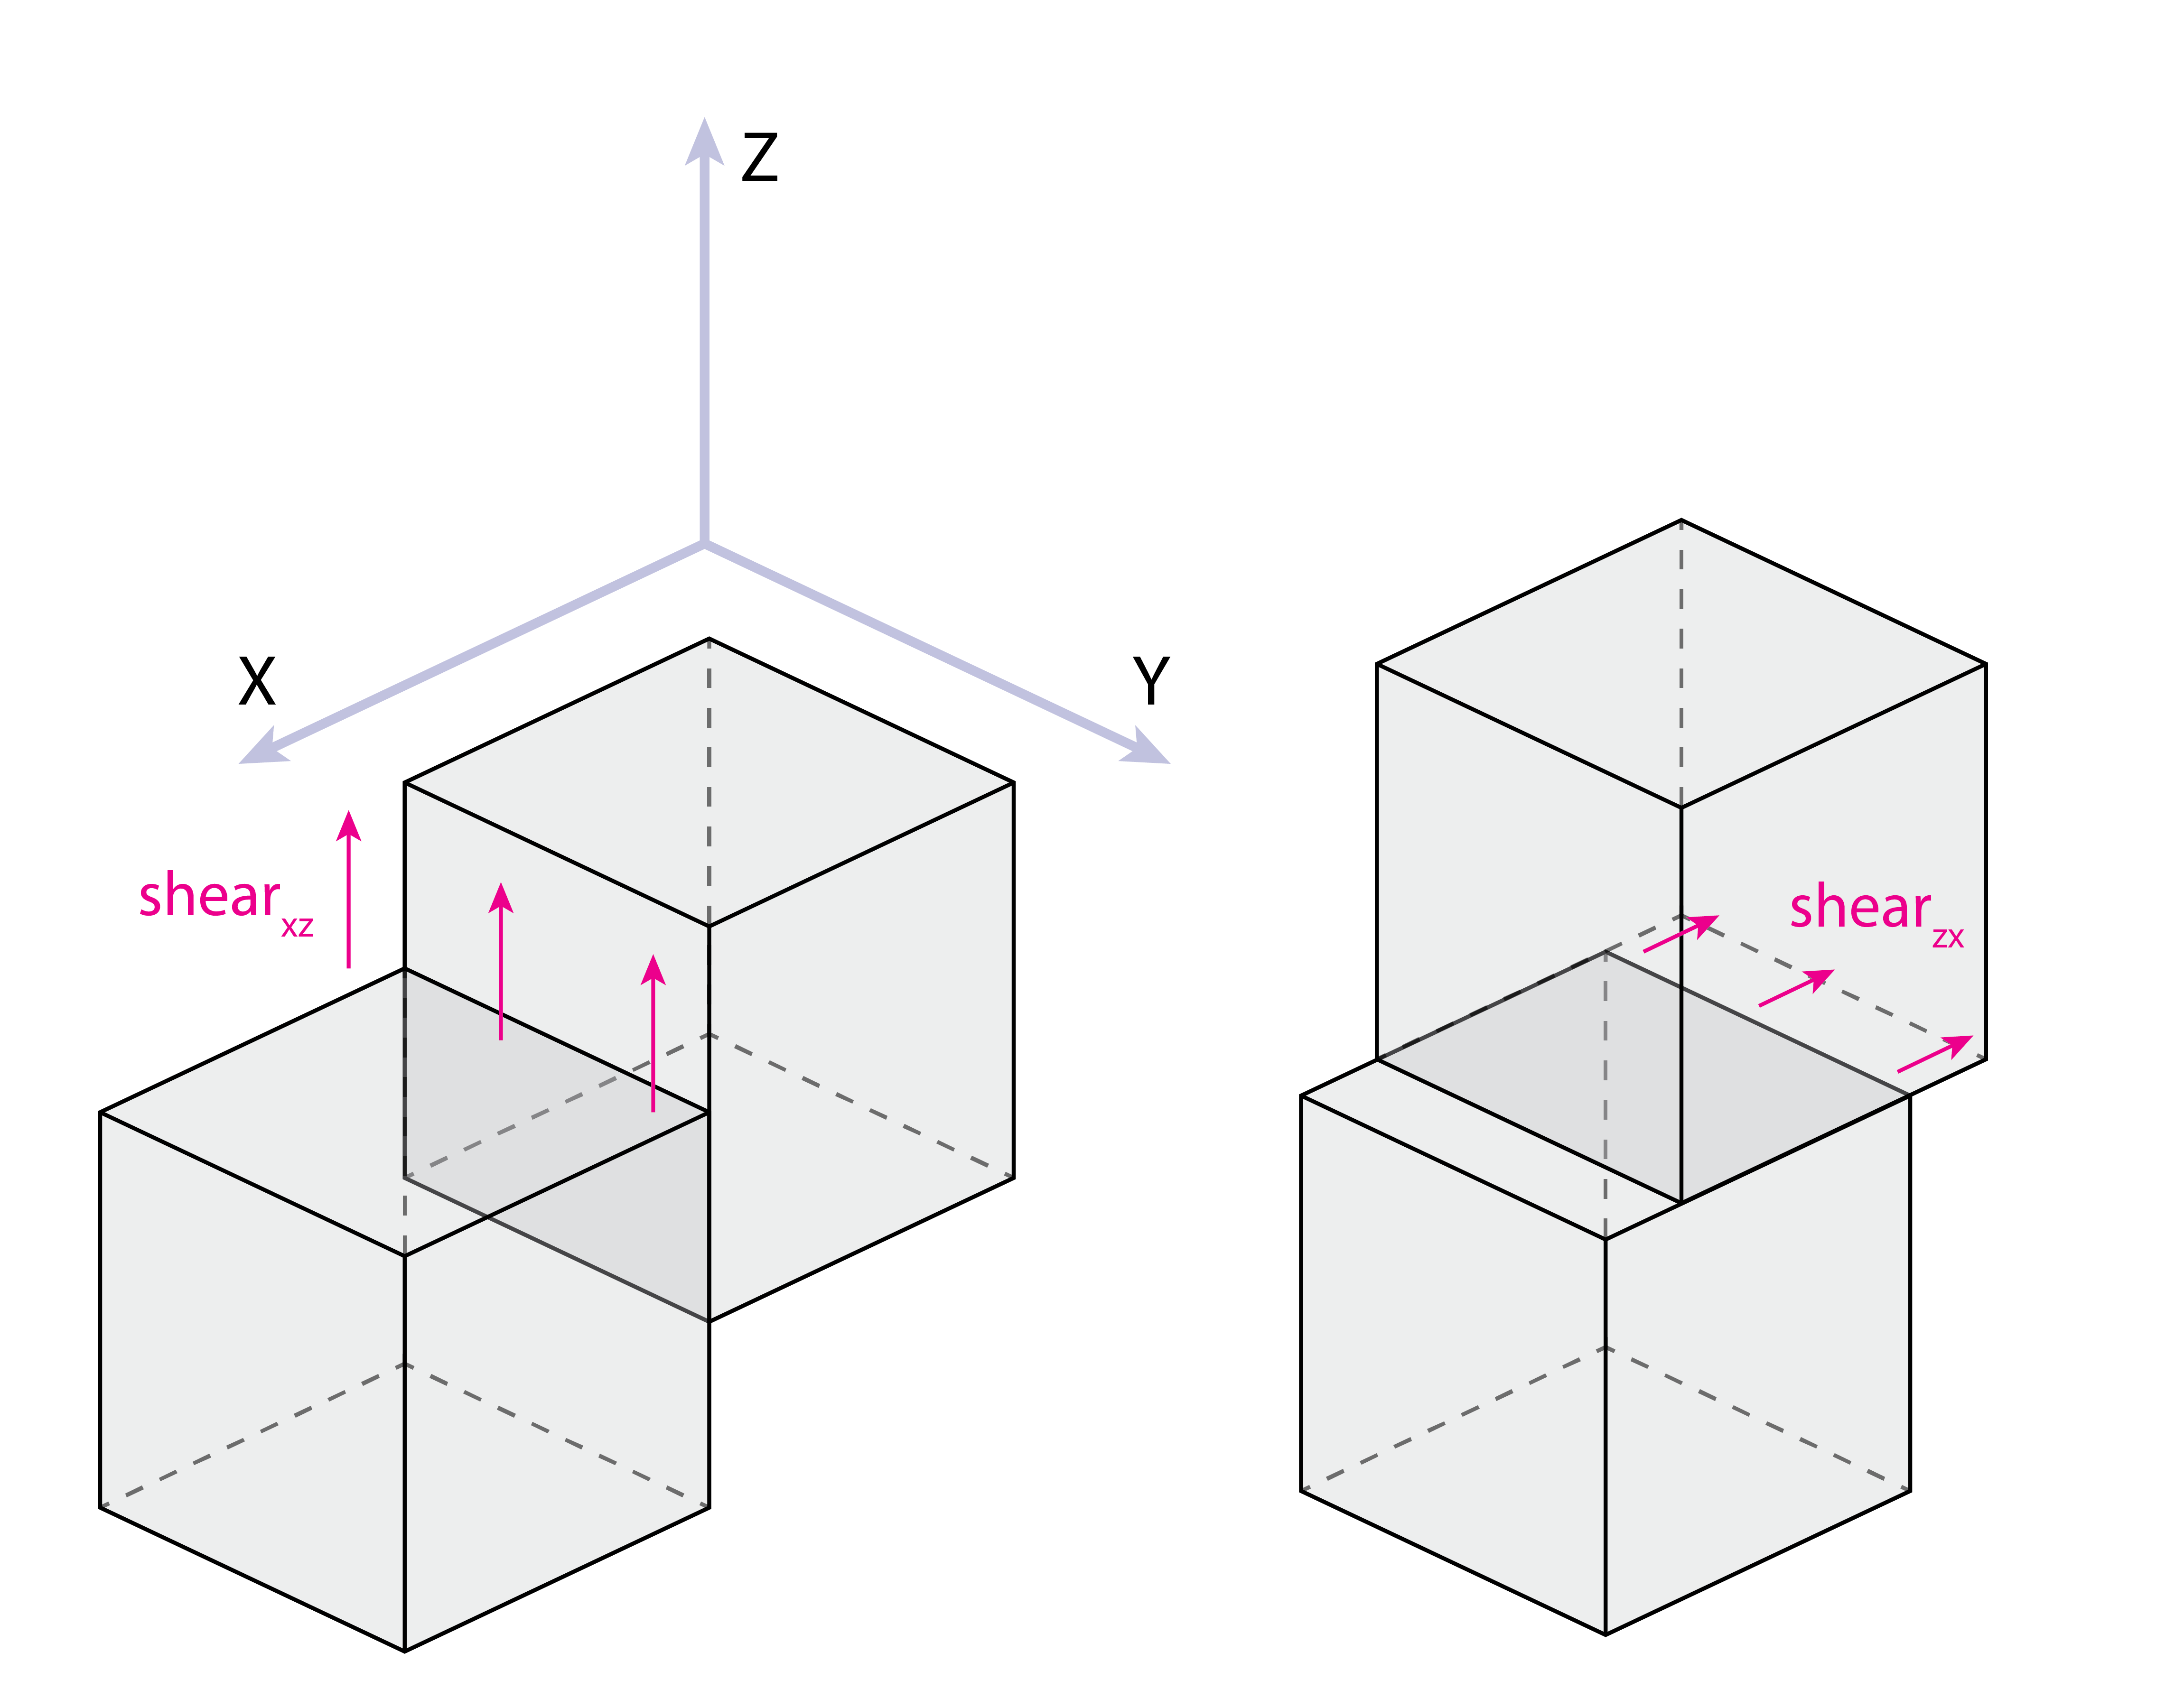
\includegraphics[width=\linewidth]{ShearDOFs.png}
  \caption{Illustration of shear subscript notation.  First subscript describes the direction of neighboring cell connection, second describes the direction of shear displacement.}
  \label{fig:ShearDOFs}
\end{figure}

The stiffness and damping constants of each cell type may be calculated from bulk properties of the constituent materials that make up the cell, or they may be measured empirically.  For example, an isotropic cell made from a bulk material with elastic modulus $E$ and shear modulus $G$ has stiffnesses along the x-axis defined by:

\begin{subequations}
\begin{align} 
\label{eq:kaxial}
k_{axial_x} &= \dfrac{EA_x}{l}\\[10pt]
\label{eq:kshear}
k_{shear_{xy}} &= \dfrac{GA_{sy}}{l}\\[10pt]
\label{eq:kbending}
k_{bending_x} &= \dfrac{EI_x}{l}??\\[10pt]
\label{eq:ktorsion}
k_{torsion_x} &= \dfrac{GJ_x}{l}??
\end{align}
\end{subequations}
\\
where $A$ is the cross sectional area and $l$ is the length of the cell.\\

 \begin{figure}
  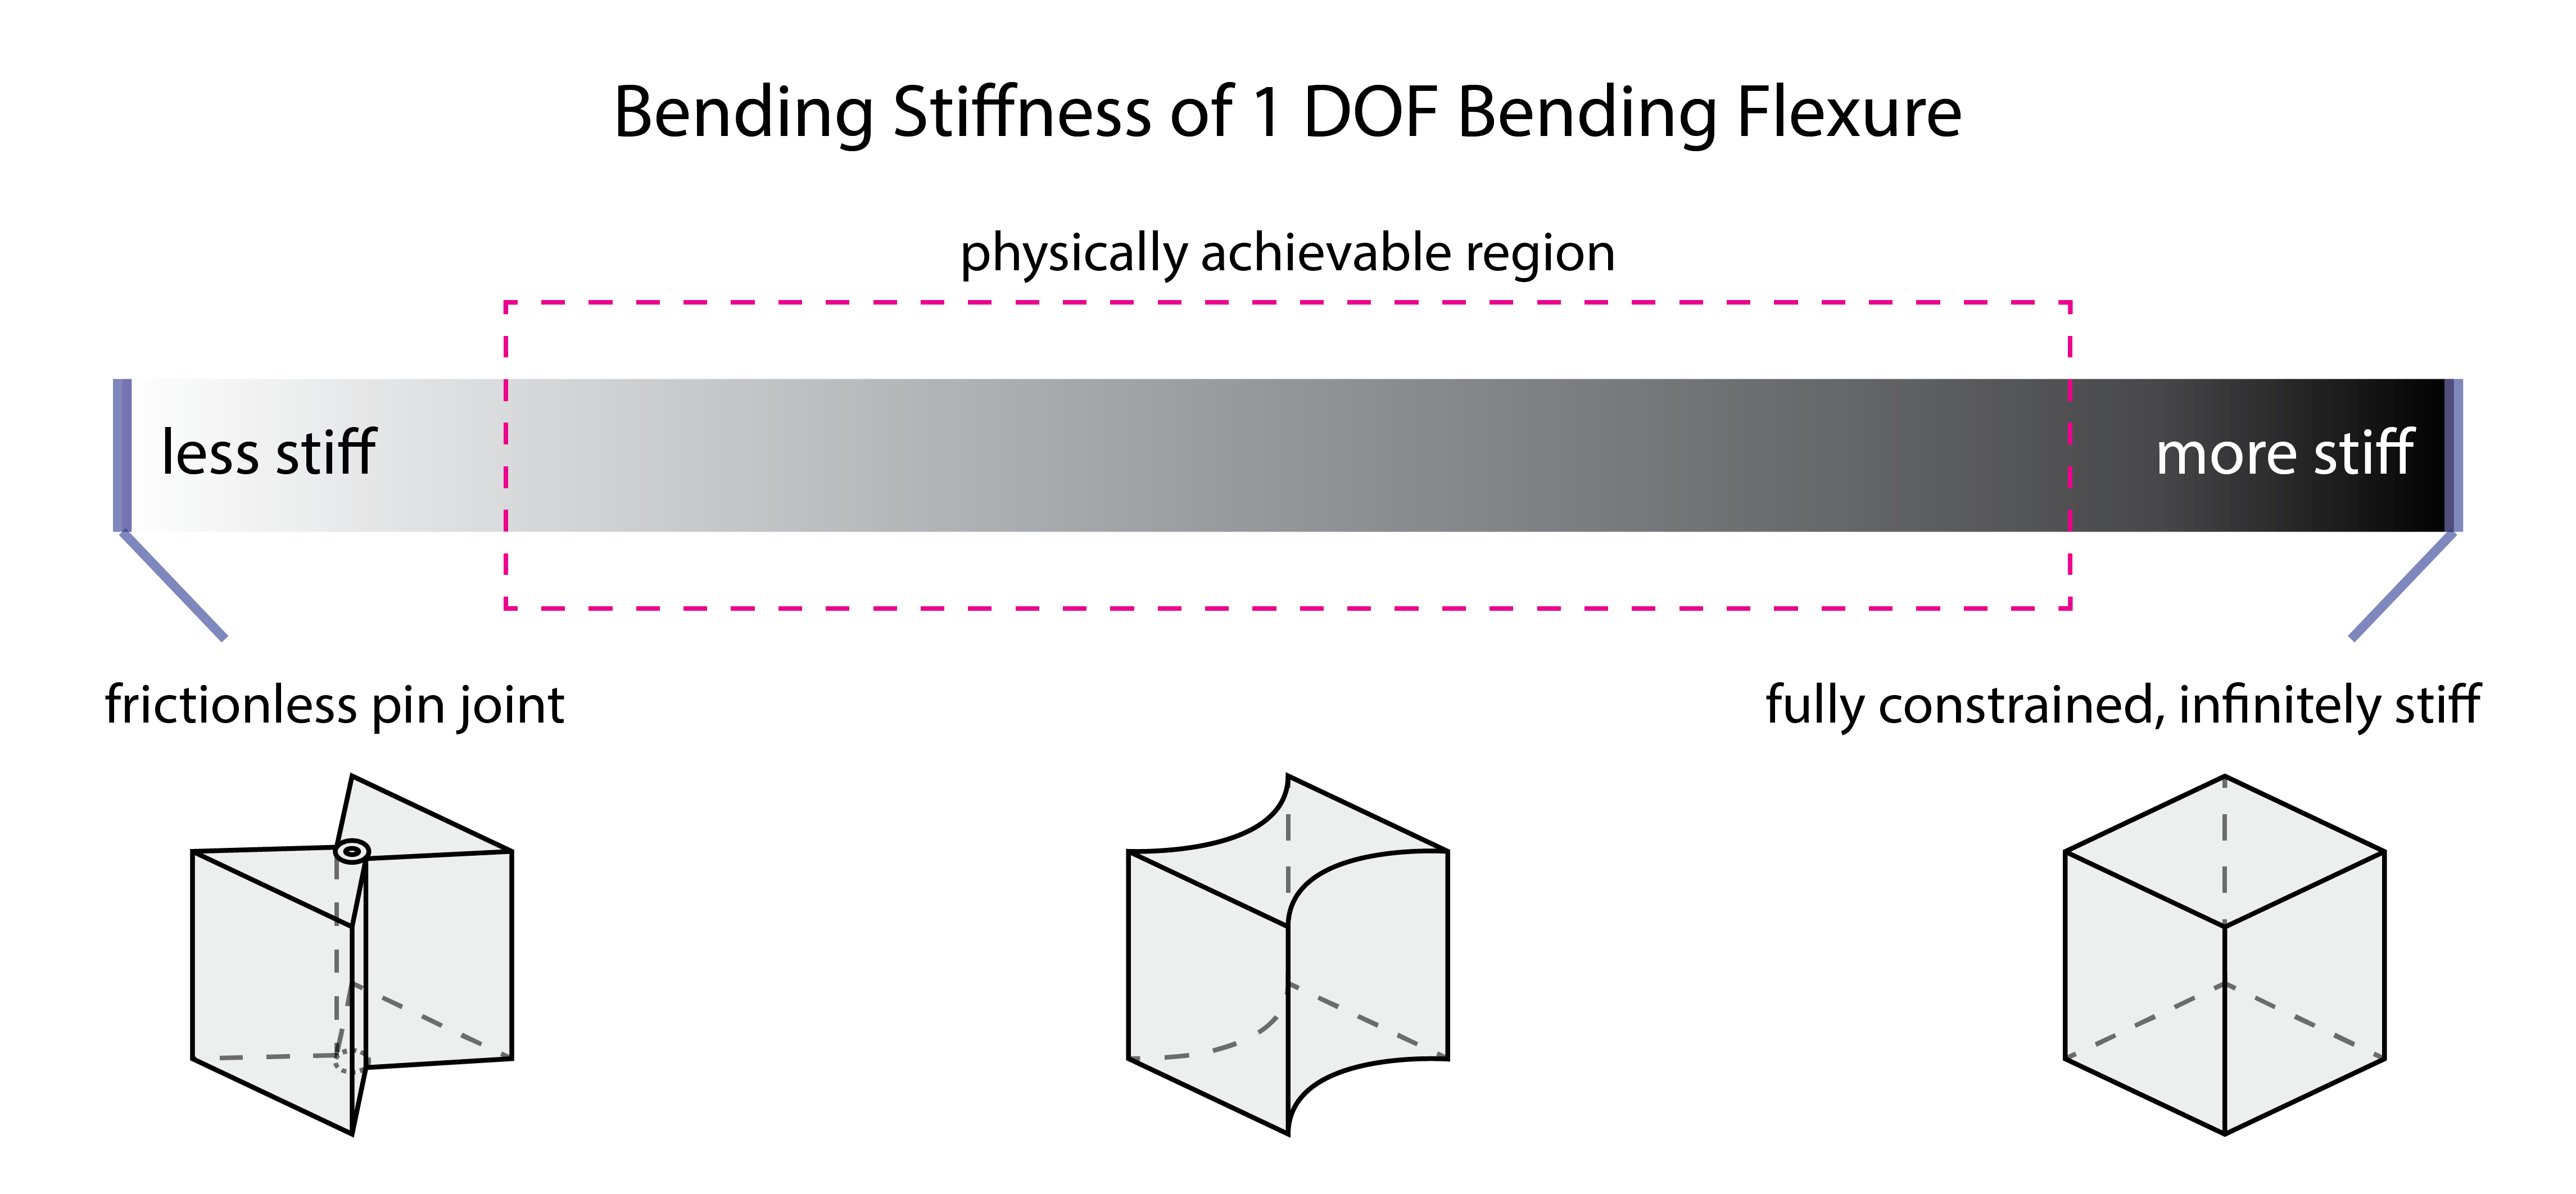
\includegraphics[width=\linewidth]{BendingStiffnessContinuoum.png}
  \caption{Continuum of bending stiffness in a 1 DOF bending flexure.  Region which can be physically achieved through existing fabrication techniques is highlighted in pink.}
  \label{fig:BendingStiffnessContinuoum}
\end{figure}

A linear scale showing the range of physically achievable 1-DOF bending cell types compared with the range of theoretically possible types is shown in Figure \ref{fig:BendingStiffnessContinuoum}.  Due to manufacturing and material constraints, we do not envision functional primitives that occupy the region near zero bending stiffness (e.g. a frictionless pin joint) or infinite bending stiffness (zero compliance material).\\

In the case that neighboring cells have different stiffness or damping constants, a composite stiffness or damping constant must be calculated in order to properly model the junction between the cells.  Composite stiffness can be calculated according to the following formula:
 \begin{equation} \label{eq:springseries}
 k_{composite} = \dfrac{2k_1k_2}{k_1+k_2}
 \end{equation}

similarly, composite damping is calculated by:
 \begin{equation} \label{eq:damperseries}
d_{composite} = \dfrac{2d_1d_2}{d_1+d_2}
 \end{equation}
 
 Equations \ref{eq:springseries} and \ref{eq:damperseries} are equivalent to the formulas for two springs or two dampers of half length in series.  This is demonstrated graphically in Figure \ref{fig:SeriesCoupling}.  Notice, for example, in the case of $k1=k2$, Equation \ref{eq:springseries} reduces to $ k_{composite} = k1 = k2$.\\
 
 \begin{figure}
  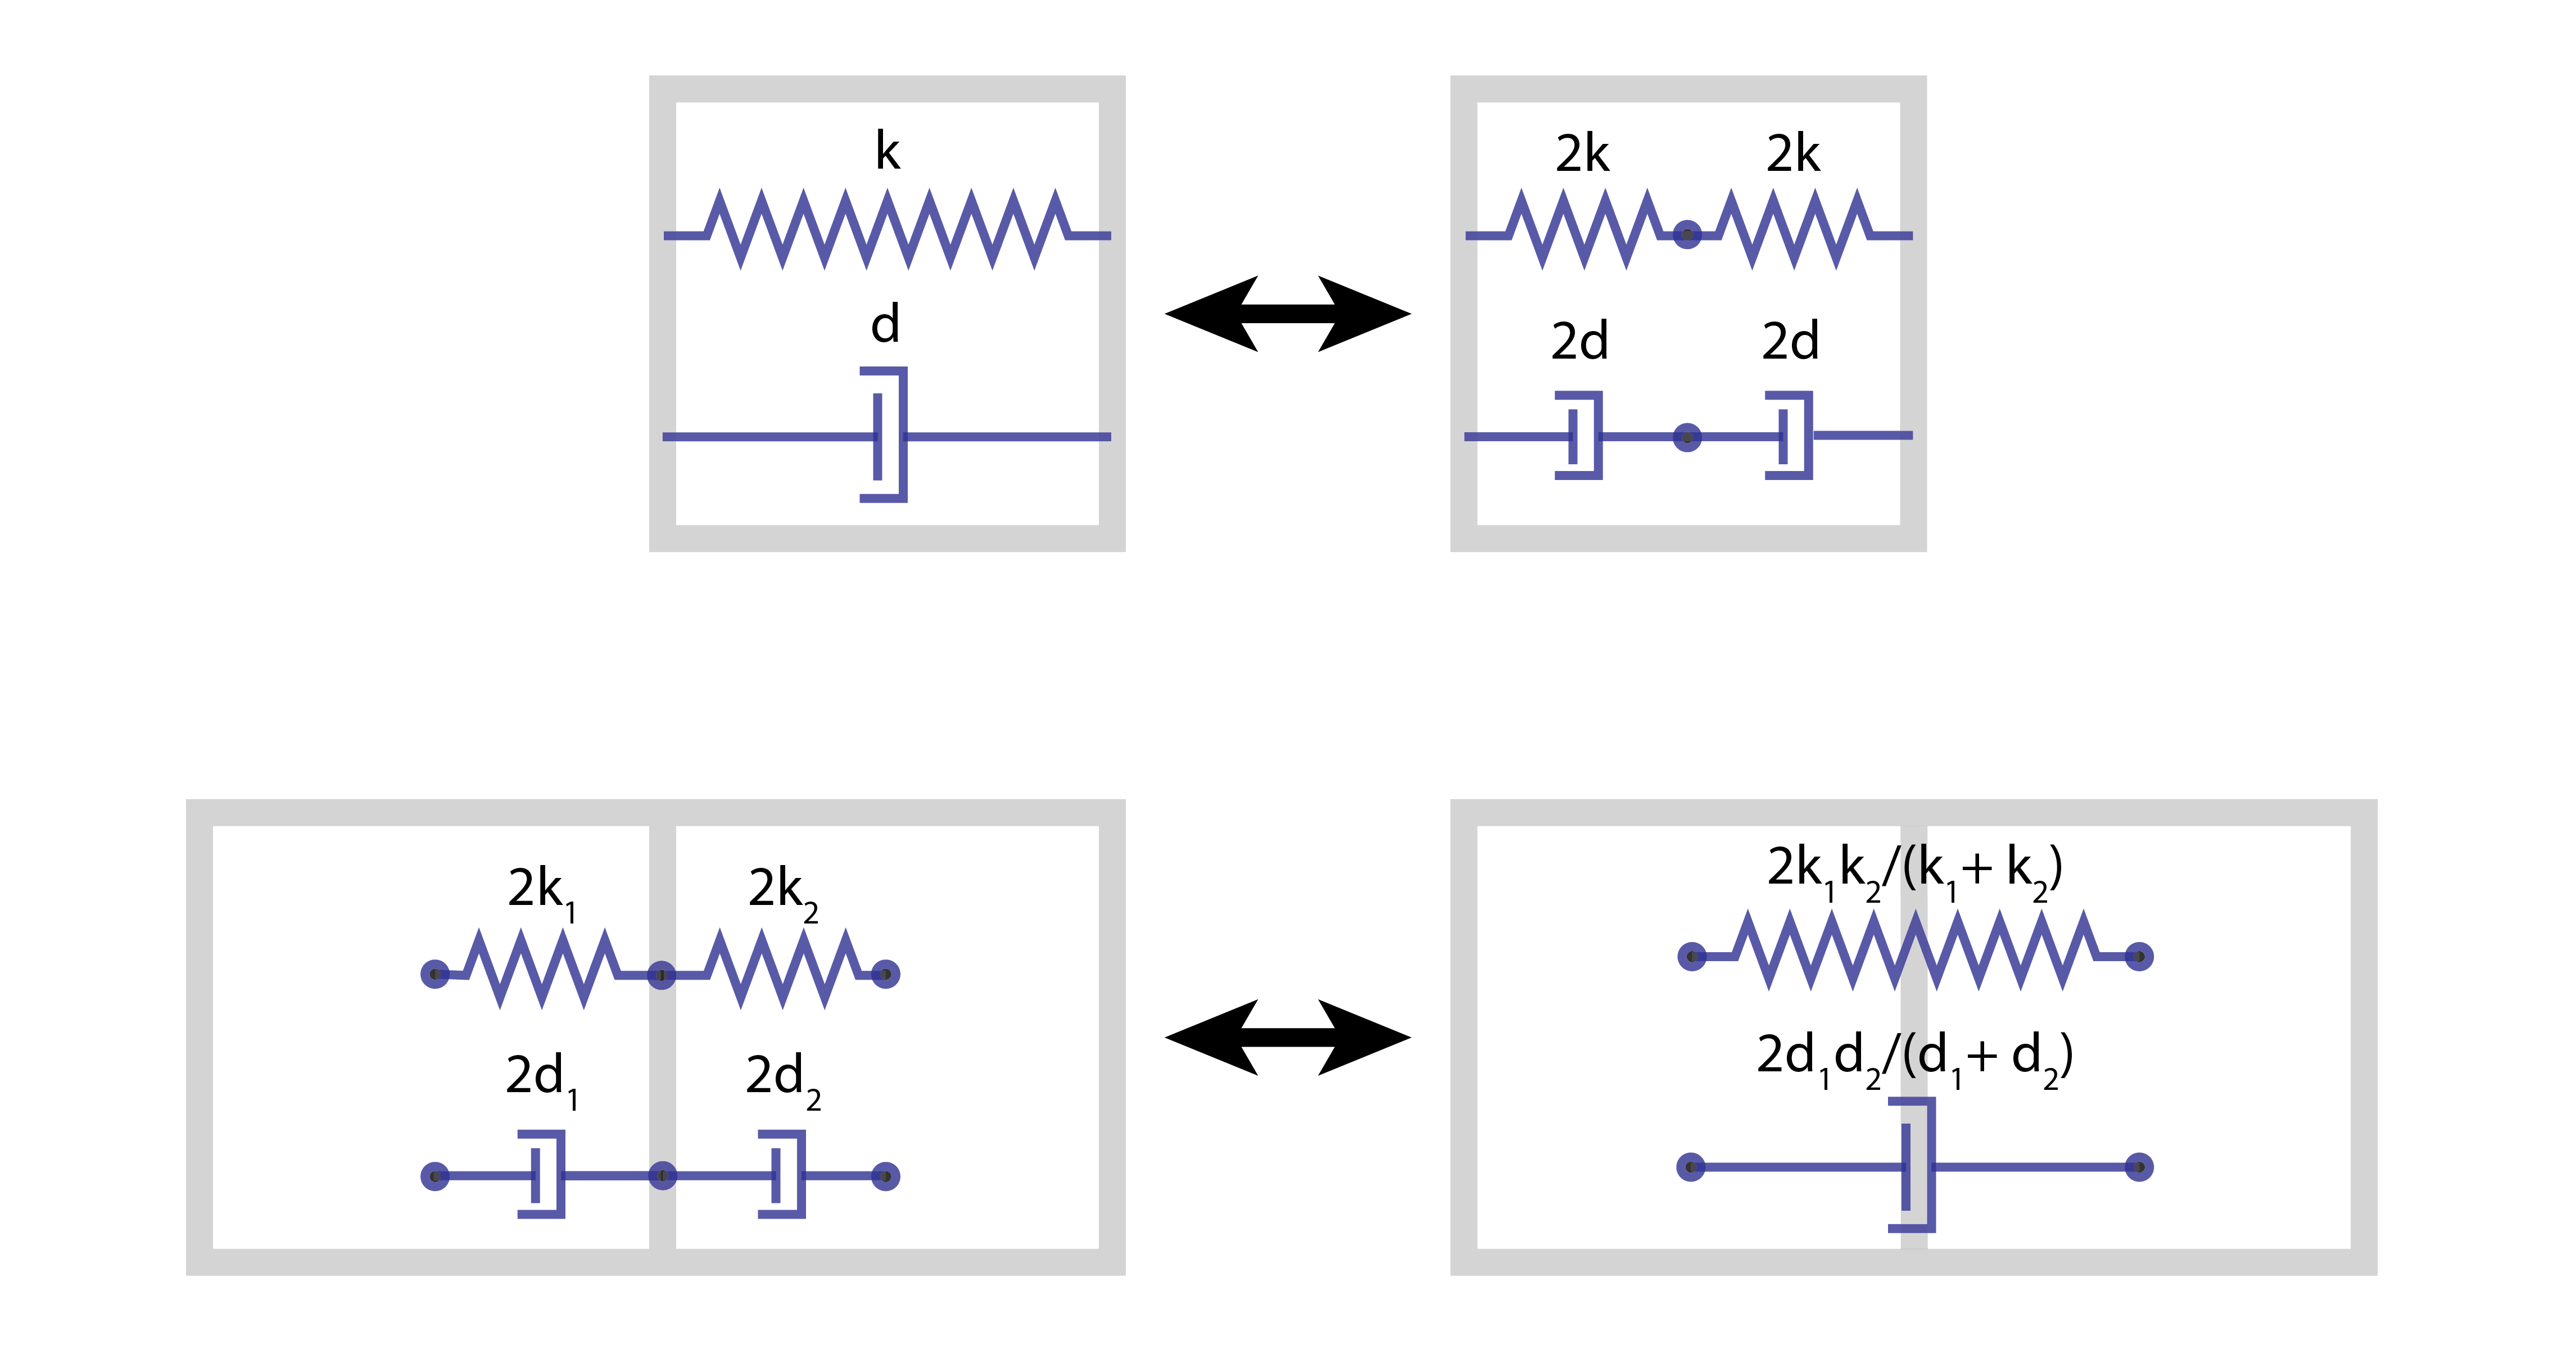
\includegraphics[width=\linewidth]{SeriesCoupling.png}
  \caption{Calculation of composite stiffness and damping of two cells with different k and d constants.}
  \label{fig:SeriesCoupling}
\end{figure}


\section{Translational Forces}

\begin{figure}
  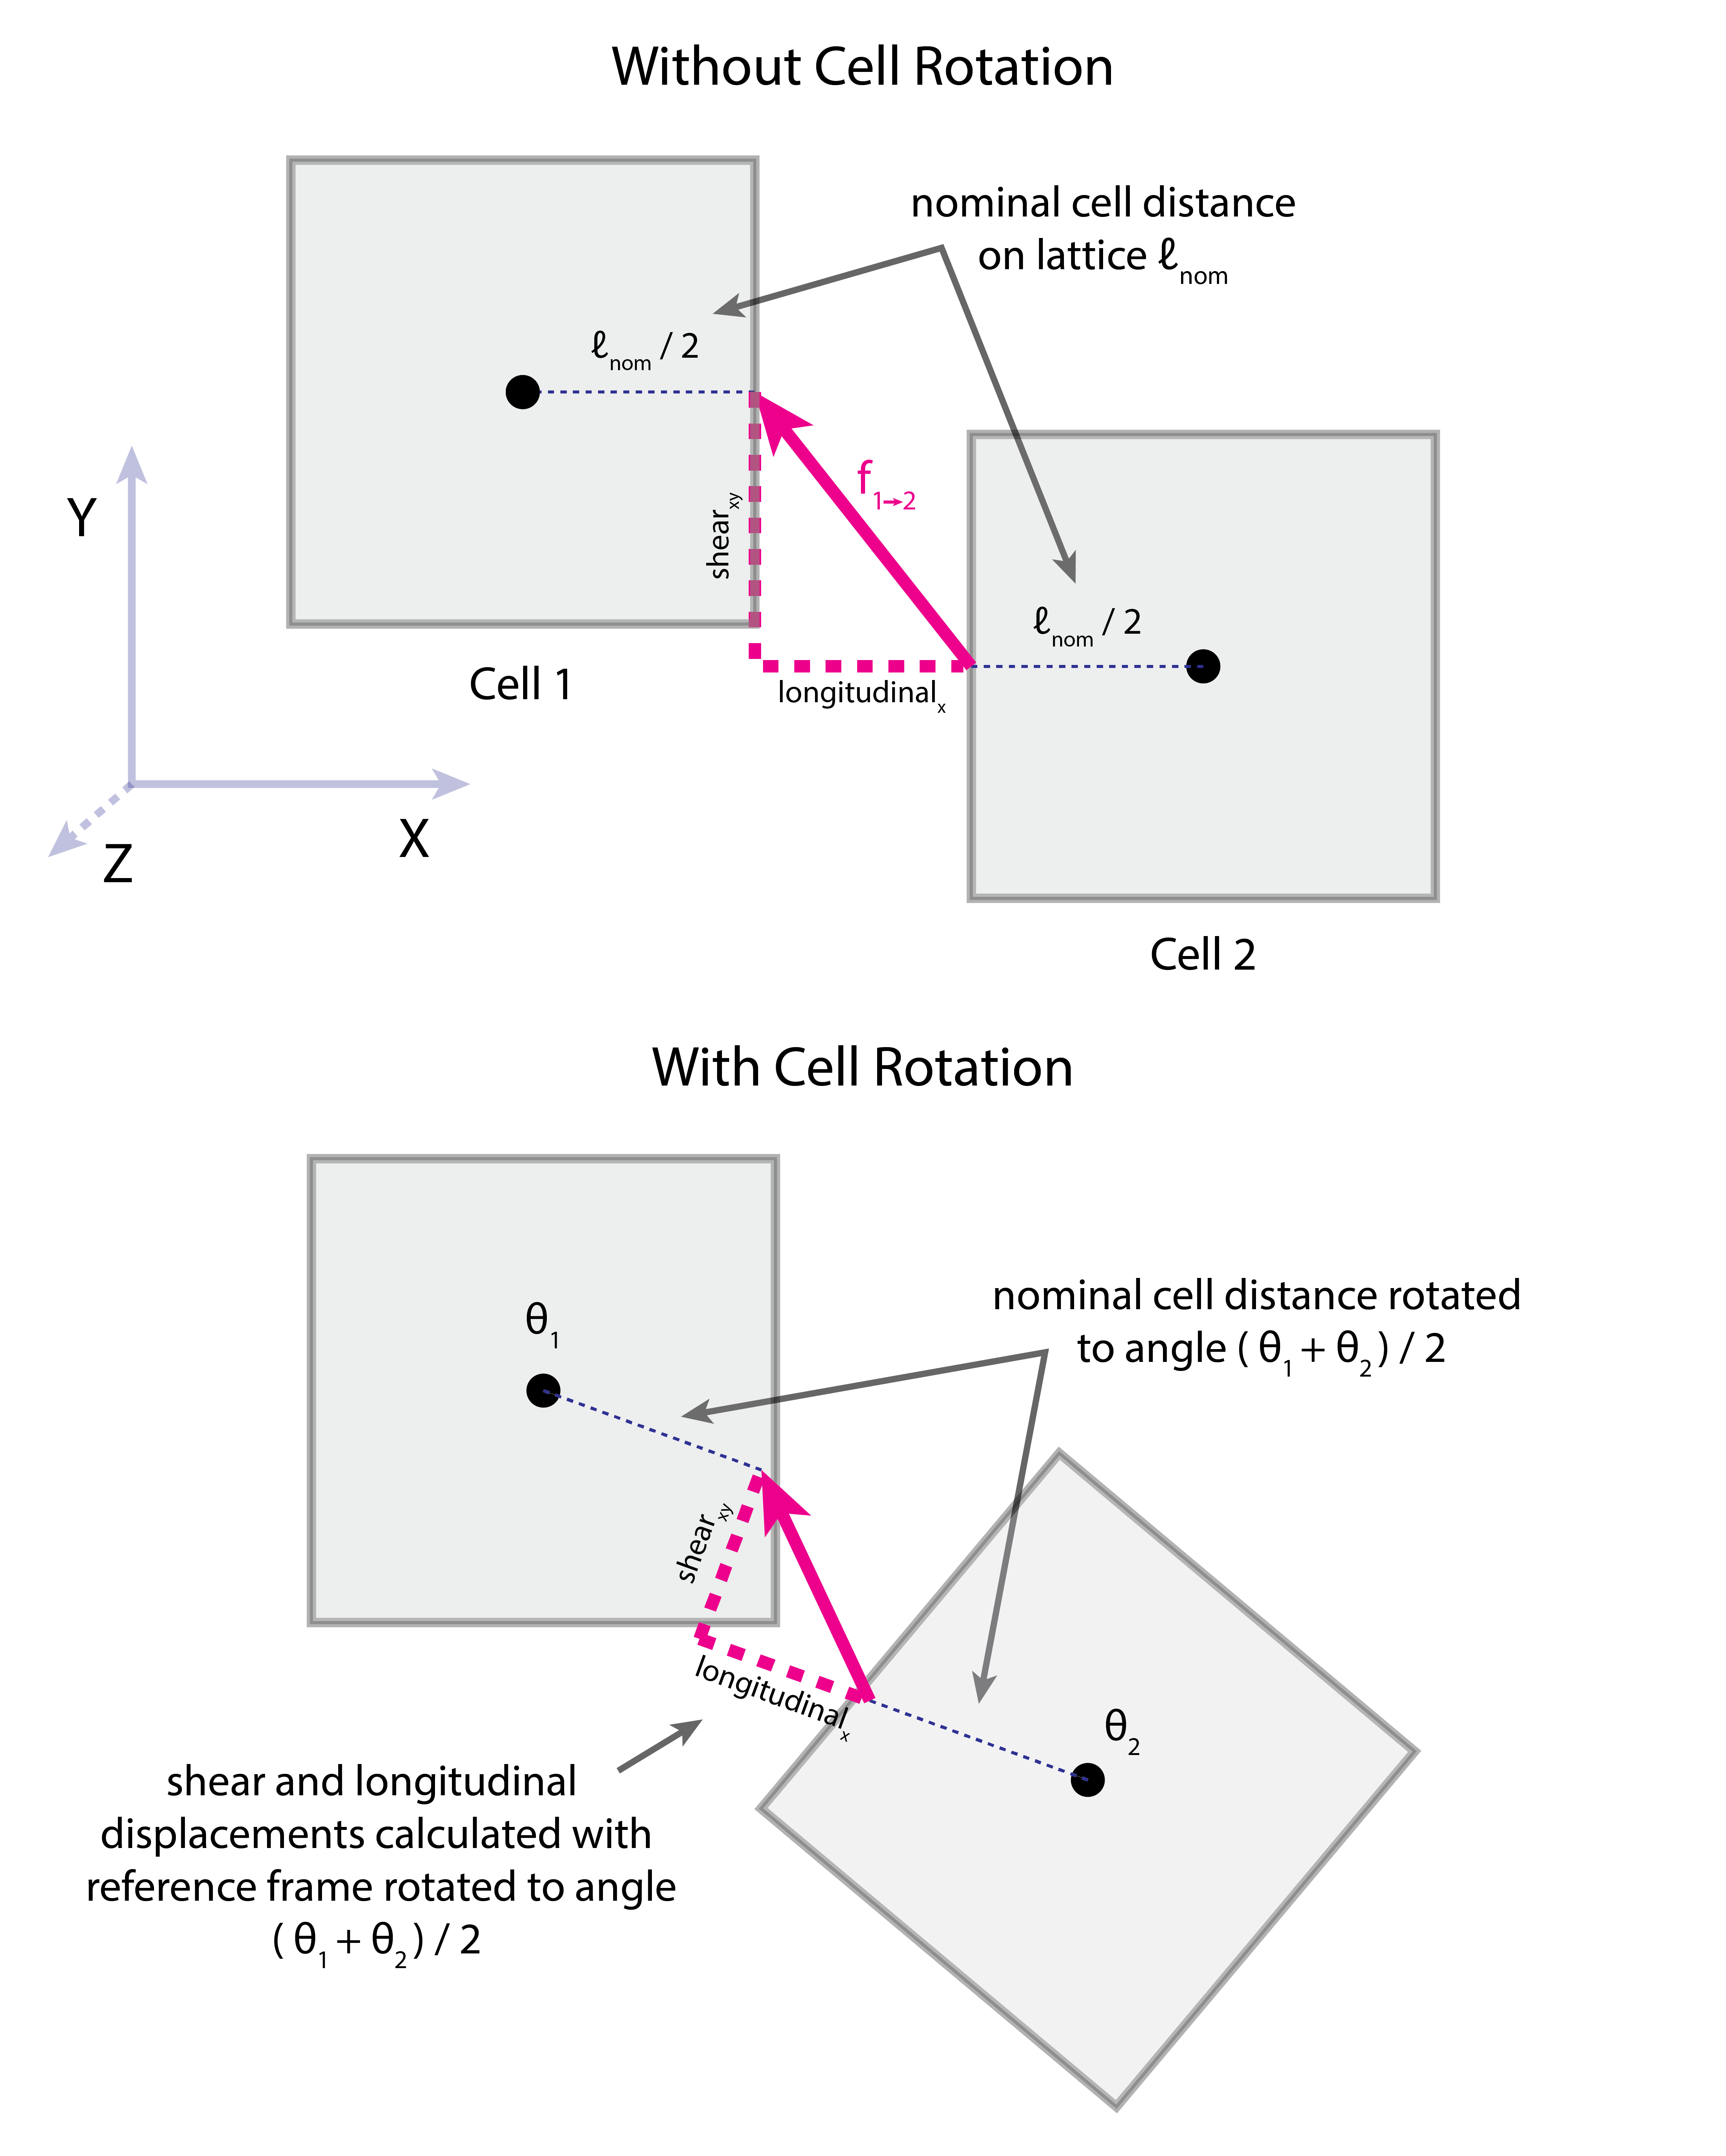
\includegraphics[width=\linewidth]{translationalSim.png}
  \caption{Diagram of translational force calculations, with and without relative rotations between cells.}
  \label{fig:translationalSim}
\end{figure}

In the simplest case without rotation, the force $\vec{F}_{1 \rightarrow 2}$ applied to cell 2 by cell 1 is given by:
\begin{equation} \label{eq:translationalForce}
\vec{F}_{1\rightarrow2} = \vec{k} \circ (\vec{p}_1 - \vec{p}_2) + \vec{d} \circ (\vec{v}_1 - \vec{v}_2)
\end{equation}

where $\vec{p}_1$ and $\vec{p}_2$ are the displacements of cell 1 and cell 2 from their nominal position in the lattice, $\vec{v}_1$ and $\vec{v}_2$ are the cells' translational velocities, $\circ$ is multiplication of two vectors by element, and $\vec{k}$ and $\vec{d}$ are 3D vectors containing the appropriate composite stiffness and damping constants for the interaction between the cells.  For example, given the scenario illustrated in Figure \ref{fig:translationalSim}, where two cells are connected along the x axis, an axial constant should be used for displacements along x and shear constants should be used for displacements along y and z:
\[ \vec{k} =  \left[ \begin{array}{ccc}
k_{axial_x}\\
k_{shear_{xy}}\\
k_{shear_{xz}}
 \end{array} \right]  
  \qquad\qquad
  \vec{d} =  \left[ \begin{array}{ccc}
d_{axial_x}\\
d_{shear_{xy}}\\
d_{shear_{xz}}
 \end{array} \right] \] 
 
If we wish to consider the orientations of the cells, denoted by the unit quaternions $q1$ and $q2$, we will need to adjust equation \ref{eq:translationalForce}. \\
  
  We can rotate a vector $\vec{v}$ in 3-space by a quaternion $q$ in 4-space:
  \begin{equation}\label{eq:hamiltonprod}
  \vec{v}_{rotated} = q*\vec{v}*q^*
  \end{equation}
  by treating $\vec{v}$ as a 4-space vector $[x, y, z, w]$ with $w=0$.  The operator $*$ denotes the Hamilton product:
  \[ a*b =  \left[ \begin{array}{ccc}
a_wb_x + a_xb_w + a_yb_z - a_zb_y\\
a_wb_y - a_xb_z + a_yb_w + a_zb_x\\
a_wb_z + a_xb_y - a_yb_x + a_zb_w\\
a_wb_w - a_xb_x - a_yb_y - a_zb_z
 \end{array} \right] \] 
 
   and $q^*$ denotes the conjugate of $q$:
    \[ q^{*} =  \left[ \begin{array}{ccc}
-q_x\\
-q_y\\
-q_z\\
q_w
 \end{array} \right] \] 
 
By performing a spherical linear interpolation (slerp) halfway between $q1$ and $q2$, we can calculate the average orientation of the two cells as a unit quaternion:
  \[ q_{avg} = slerp(q_{1}, q_{2}; 0.5) \]
  
Using $q_{avg}$, we can rotate the stiffness and damping vectors from Equation \ref{eq:translationalForce} into this average reference frame, and substitute the rotated vectors back into equation \ref{eq:translationalForce}:
\begin{subequations}
\begin{align}
\label{eq:krotated}
 \vec{k}_{rot} &= (q_{avg}*\vec{k}*q_{avg}^*)\\
 \label{eq:drotated}
  \vec{d}_{rot} &= (q_{avg}*\vec{d}*q_{avg}^*)
  \end{align}
  \end{subequations}
  \begin{equation} \label{eq:translationalForceRotStep}
 \vec{F}_{1\rightarrow2} = \vec{k}_{rot} \circ (\vec{p}_1 - \vec{p}_2) + \vec{d}_{rot} \circ (\vec{v}_1 - \vec{v}_2)
 \end{equation}
 
Finally, we need to make an adjustment to the nominal differential position between the cells, indicated in Figure \ref{fig:translationalSim}.  The form above assumes the nominal distance between the centers of the cells is the unrotated distance from cells 2 to cell 1 in their initial lattice configuration, $\vec{l}_{nom21}$:
\begin{equation}\label{eq:lnominal}
\vec{l}_{nom21} = \vec{p}_{abs2}-\vec{p}_{abs1}
\end{equation}
 
 where $\vec{p}_{abs}$ is the absolute position of a cell in the world reference frame.
 Rotating $\vec{l}_{nom}$ into the average rotational reference frame of the two cells gives
 \[\vec{l}_{rot21} = q_{avg}*\vec{l}_{nom21}*q_{avg}^*\]
 
introducing this correction to Equation \ref{eq:translationalForceRotStep} gives the final form:
 \begin{equation} \label{eq:translationalForceRot}
  \vec{F}_{1\rightarrow2} = \vec{k}_{rot} \circ (\vec{p}_1 - \vec{p}_2 + \vec{l}_{nom21}-\vec{l}_{rot21}) + \vec{d}_{rot} \circ (\vec{v}_1 - \vec{v}_2)
  \end{equation}

The force $\vec{F}_{2\rightarrow1}$ exerted on cell 2 by cell 1 is equal in magnitude to $\vec{F}_{1\rightarrow2}$ and opposite in direction:
 \begin{equation} \label{eq:translationalEqOpp}
  \vec{F}_{2\rightarrow1} = -\vec{F}_{1\rightarrow2} = \vec{k}_{rot} \circ (\vec{p}_1 - \vec{p}_2 + \vec{l}_{nom12}-\vec{l}_{rot12}) + \vec{d}_{rot} \circ (\vec{v}_1 - \vec{v}_2)
  \end{equation}

Only $\vec{F}_{1\rightarrow2}$ is indicated with a solid pink arrow in Figure \ref{fig:translationalSim}.\\

Dividing by the mass, we can calculate the acceleration of cells 1 and 2 due to interactions between them:

 \[ \vec{a}_{1\rightarrow2} = \dfrac{\vec{F}_{1\rightarrow2}}{m_2} 
  \qquad\qquad
   \vec{a}_{2\rightarrow1} = \dfrac{\vec{F}_{2\rightarrow1}}{m_1} 
  \]

\section{Rotational Forces}

So far, this model uses shear and axial stiffness and damping constants to compute the translational interactions between neighboring cells in 3D.  In order to incorporate bending and torsional forces, we must develop a method of for cells to apply torques to one another.  These torques result in rotational motion of a cell about its center of mass (assumed to be the center of the cell).\\

\begin{figure}
  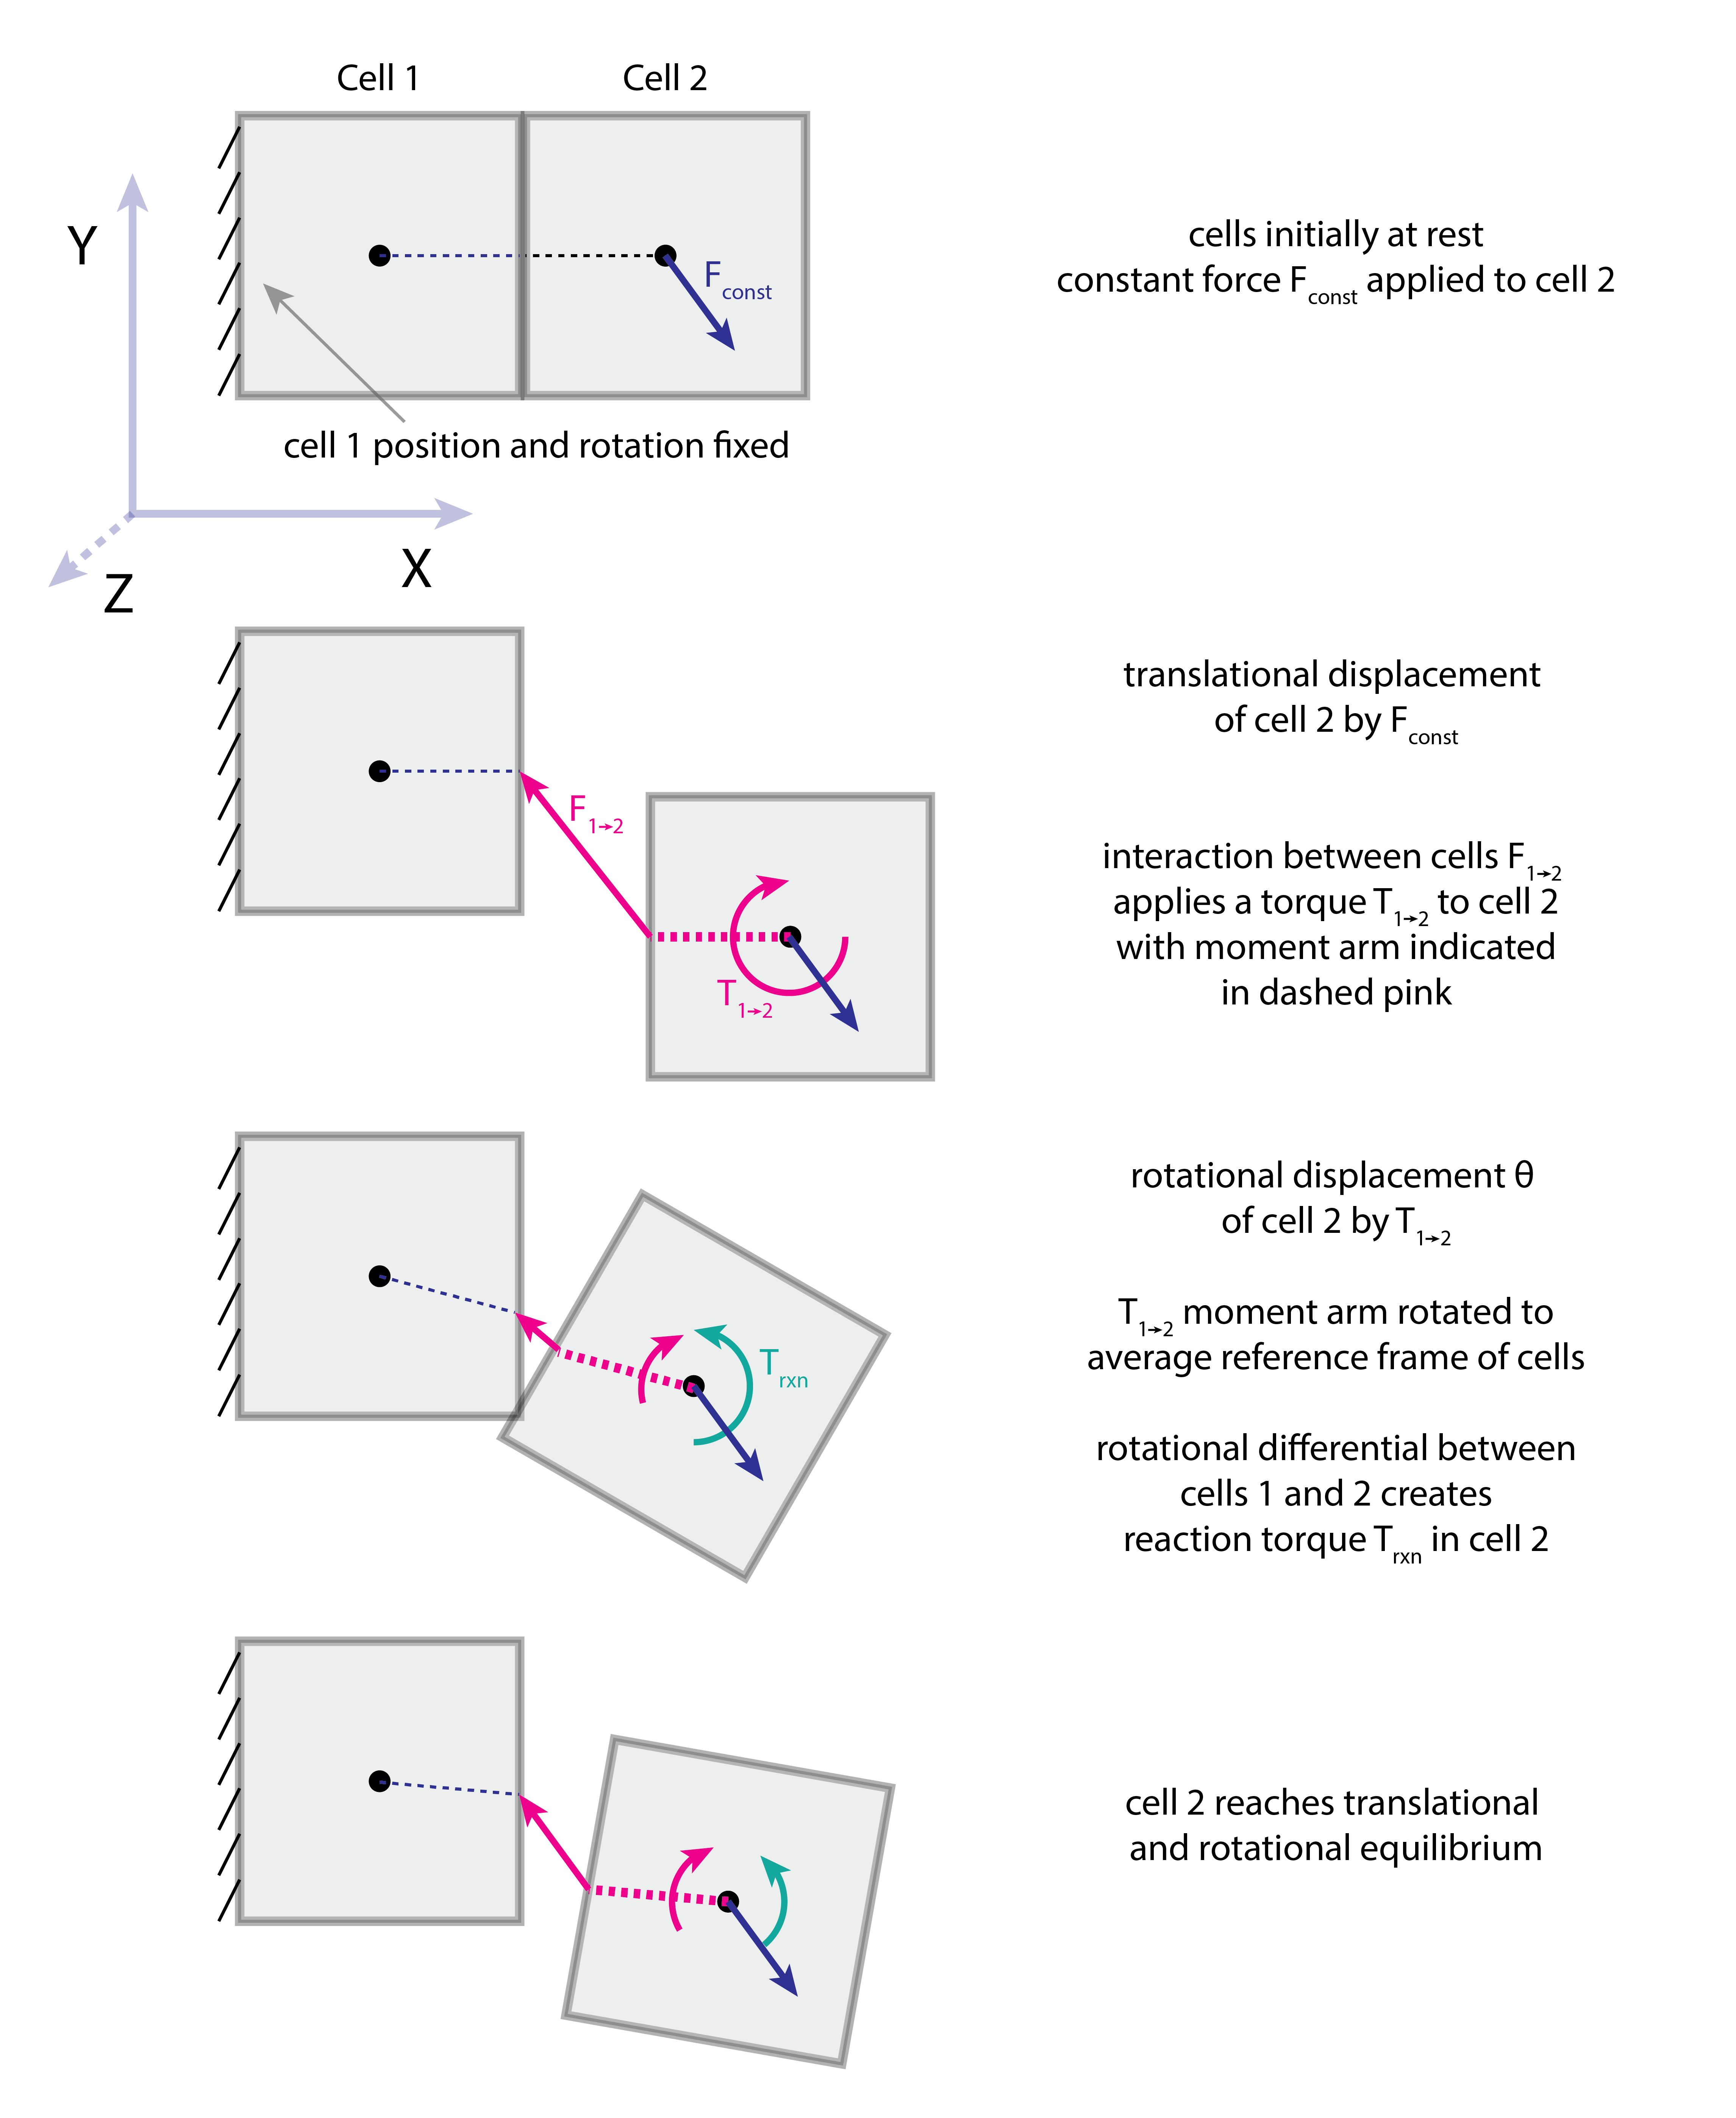
\includegraphics[width=\linewidth]{rotationalSim.png}
  \caption{Diagram of translational and rotational forces between cells.  Translational forces due to shearing cause a torque in cell 2 ($T_{1\rightarrow2}$).  Relative rotation between the cells induces a reaction torque ($T_{rxn}$).}
  \label{fig:rotationalSim}
\end{figure}

A sketch of the translational and rotational model for cell interaction is shown in Figure \ref{fig:rotationalSim}.  In this model, we consider the fact that shear and axial forces between cells are not applied directly to the center of mass of a cell, but rather at some moment arm from the center of mass.  We define the moment arm $\vec{r}_{moment2}$ of cell 2 to be half the nominal distance from cell 2 to cell 1, rotated to the average reference frame of the two cells:

\[ \vec{r}_{moment} = \dfrac{\vec{l}_{rot21}}{2}\]

Then the torque $\vec{T}_{1\rightarrow2}$ can be calculated by the cross product:
\begin{equation}\label{eq:moment1to2}
\vec{T}_{1\rightarrow2} =  \vec{r}_{moment} \times \vec{F}_{1\rightarrow2}
\end{equation}

If we stop now, we have set up a simulation of an arbitrary linkage of cells tied together with frictionless, spherical joints at their centers of mass.\\

Next we'll add in bending and torsional stiffness, which create reaction forces that counteract relative rotations between cells ($T_{rxn}$ in Figure \ref{fig:rotationalSim}).  For neighboring cells oriented along the x axis, we have composite stiffness and damping vectors:
\[ \vec{k} =  \left[ \begin{array}{ccc}
k_{torsion_x}\\
k_{bending_{y}}\\
k_{bending_{z}}
 \end{array} \right]  
  \qquad\qquad
  \vec{d} =  \left[ \begin{array}{ccc}
d_{torsion_x}\\
d_{bending_{y}}\\
d_{bending_{z}}
 \end{array} \right] \] 

Then we rotate the composite stiffness and damping constants into the average reference frame between the cells as we did in Equations \ref{eq:krotated} and \ref{eq:drotated} to get $\vec{k}_{rot}$ and $\vec{d}_{rot}$.\\

Next we calculate the angular displacement and relative angular velocity between the two cells.  We have to be careful in this step to remember that angular velocities (and torques) are vectors in cartesian space, but euler rotations ($\vec{\theta}$) are vectors in spherical space.  So while vector addition and subtraction of angular velocities is valid:
\[ \vec{\omega}_{diff} = \vec{\omega}_1 - \vec{\omega}_2 \]

Vector addition and subtraction of euler rotations is not valid (though it might be ok for small angles):
\[ \vec{\theta}_{diff} \neq \vec{\theta}_1 - \vec{\theta}_2 \]

Instead, we'll use the two cells' quaternions to calculate the axis ($\vec{A}_{\theta}$) and angle of rotation ($\alpha_{\theta}$) from cell 2 to cell 1:
\begin{equation}\label{eq:qdiff}
q_{diff} = q_1^{*}*q_2 
\end{equation}
\[ \alpha_{\theta} = 2*acos(q_{diff_w}) \]

(if $\alpha$ == 0 then the axis does not matter, we can pick something arbitrary)
\[ A_{\theta} = \dfrac{1}{\sqrt{1-q_{diff_w}^2}} \left[ \begin{array}{ccc}
q_{diff_x}\\
q_{diff_y}\\
q_{diff_z}
 \end{array} \right] \]
 
$A_{\theta}$,  $\alpha_{\theta}$, $\omega_1$, and $\omega_2$ are used to calculate reaction torque of cell 2 ($T_{2_{rxn}}$), following a similar spring/damper setup as we used in Equation \ref{eq:translationalForceRot}:
\begin{equation}\label{eq:reactiontorque}
\vec{T}_{2_{rxn}} = \vec{k}_{rot} \circ (\alpha_{\theta} \vec{A}_{\theta}) + \vec{d}_{rot} \circ (\omega_1-\omega_2)
\end{equation}

The total torque on cells 2 is the sum of the torque applied by shear and axial interactions with cell 1 (Equation \ref{eq:moment1to2}) and the reaction force of cell 2 (Equation \ref{eq:reactiontorque}):
\begin{equation}\label{eq:torqueEquation}
\vec{T}_2 = \vec{T}_{1\rightarrow2} + \vec{T}_{2_{rxn}}
\end{equation}

The torque on cell 1 from the interaction with cell 2 is equal in magnitude and opposite in direction:
\[ \vec{T}_1 = -\vec{T}_{1\rightarrow2} - \vec{T}_{2_{rxn}}  = \vec{T}_{2\rightarrow1} + \vec{T}_{1_{rxn}}\]

To calculate angular acceleration ($\vec{\dot{\omega}}$), we divide by moment of inertia.  For a 3D rectangular cell with sides $l_x$, $l_y$, $l_z$ and mass $m$, the tensor moment of inertia is given by:
\[ I_{inertia} = \dfrac{m}{12} \left[ \begin{array}{ccc}
l_y^2+l_z^2 & 0 & 0\\
0 & l_x^2+l_z^2 & 0\\
0 & 0 & l_x^2+l_y^2
 \end{array} \right] \]
 
 where:
 \[ \vec{T} = I_{inertia}\vec{\dot{\omega}} \]
  \[ \vec{\dot{\omega}}  = I_{inertia}^{-1}\vec{T} \]
  \[ I_{inertia}^{-1} = \dfrac{12}{m} \left[ \begin{array}{ccc}
\dfrac{1}{l_y^2+l_z^2} & 0 & 0\\
0 & \dfrac{1}{l_x^2+l_z^2} & 0\\
0 & 0 & \dfrac{1}{l_x^2+l_y^2}
 \end{array} \right] \]
 
For cells 1 and 2:
 \[ \vec{\dot{\omega}}_1 = \dfrac{12}{m_1} \vec{T}_1 \circ 
 \left[ \begin{smallmatrix}
\tfrac{1}{l_y^2+l_z^2}\\
\tfrac{1}{l_x^2+l_z^2}\\
\tfrac{1}{l_x^2+l_y^2}
 \end{smallmatrix} \right] 
  \qquad\qquad
   \vec{\dot{\omega}}_2 = \dfrac{12}{m_2} \vec{T}_2 \circ
   \left[ \begin{smallmatrix}
\tfrac{1}{l_y^2+l_z^2}\\
\tfrac{1}{l_x^2+l_z^2}\\
\tfrac{1}{l_x^2+l_y^2}
 \end{smallmatrix} \right] 
  \]
  
  where, again, $\circ$ is multiplication of two vectors by element.

\section{Actuation}

Mechanical actuation is achieved by changing the nominal translation/rotation of a particular degree of freedom.  For example if the nominal distance ($l_{nom21}$ from Equation \ref{eq:lnominal}) between two cells oriented along the x axis at a distance $l$ is given by:
\[ \vec{l}_{nom21} =  \left[ \begin{array}{ccc}
l\\
0\\
0
 \end{array} \right] \]
 
 An axial actuator cell with strain $\Delta\epsilon$ would be modeled with the following nominal distance to its neighbor:
 \[ \vec{l}_{nom21} =  \left[ \begin{array}{ccc}
l+\tfrac{1}{2}\Delta\epsilon\\
0\\
0
 \end{array} \right] \]
 
 where the factor of $\tfrac{1}{2}$ comes from the strain being split between the neighbor to the +x direction and the -x direction equally.\\
 
 For a shear actuator, with shearing strain $\Delta\epsilon$ occurring in the y direction, the nominal distance to the neighboring cells becomes:
  \[ \vec{l}_{nom21} =  \left[ \begin{array}{ccc}
l\\
\tfrac{1}{2}\Delta\epsilon\\
0
 \end{array} \right] \]
 
 And, similarly, for a shear actuator in the z direction:
   \[ \vec{l}_{nom21} =  \left[ \begin{array}{ccc}
l\\
0\\
\tfrac{1}{2}\Delta\epsilon
 \end{array} \right] \]
 
 For rotations, we subtract the actuated angular offset in the calculation of the difference in orientation between two cells (Equation \ref{eq:qdiff}):
\[ q_{diff} = q_{actuated}^**(q_1^{*}*q_2)\]

where the actuator strain between two cells is given by the 3D euler angle $\phi$ and:
\[ q_{actuated} = \left[ \begin{array}{ccc}
sin(\phi_x) * cos(\phi_y) * cos(\phi_z) + cos(\phi_x) * sin(\phi_y) * sin(\phi_z)\\
cos(\phi_x) * sin(\phi_y) * cos(\phi_z) - sin(\phi_x) * cos(\phi_y) * sin(\phi_z)\\
cos(\phi_x) * cos(\phi_y) * sin(\phi_z) + sin(\phi_x) * sin(\phi_y) * cos(\phi_z)\\
cos(\phi_x) * cos(\phi_y) * cos(\phi_z) - sin(\phi_x) * sin(\phi_y) * sin(\phi_z)
 \end{array} \right]
\]

For a torsional actuator with angular strain $\Delta\epsilon$:
\[ \phi = \left[ \begin{array}{ccc}
\tfrac{1}{2}\Delta\epsilon\\
0\\
0
 \end{array} \right]
\]

And for a y-axis bending actuator:
\[ \phi = \left[ \begin{array}{ccc}
0\\
\tfrac{1}{2}\Delta\epsilon\\
0
 \end{array} \right]
\]

And, similarly, for a z-axis bending actuator:
\[ \phi = \left[ \begin{array}{ccc}
0\\
0\\
\tfrac{1}{2}\Delta\epsilon
 \end{array} \right]
\]

\section{Sources of Error}

\subsection{Numerical Time Integration}

Numerical time integration usually introduces error into the system's state.  For undamped, underdamped, or very stiff oscillating systems, this error can lead to numerical instability (Figure \ref{fig:numericalInstability}).\\

\begin{figure}
  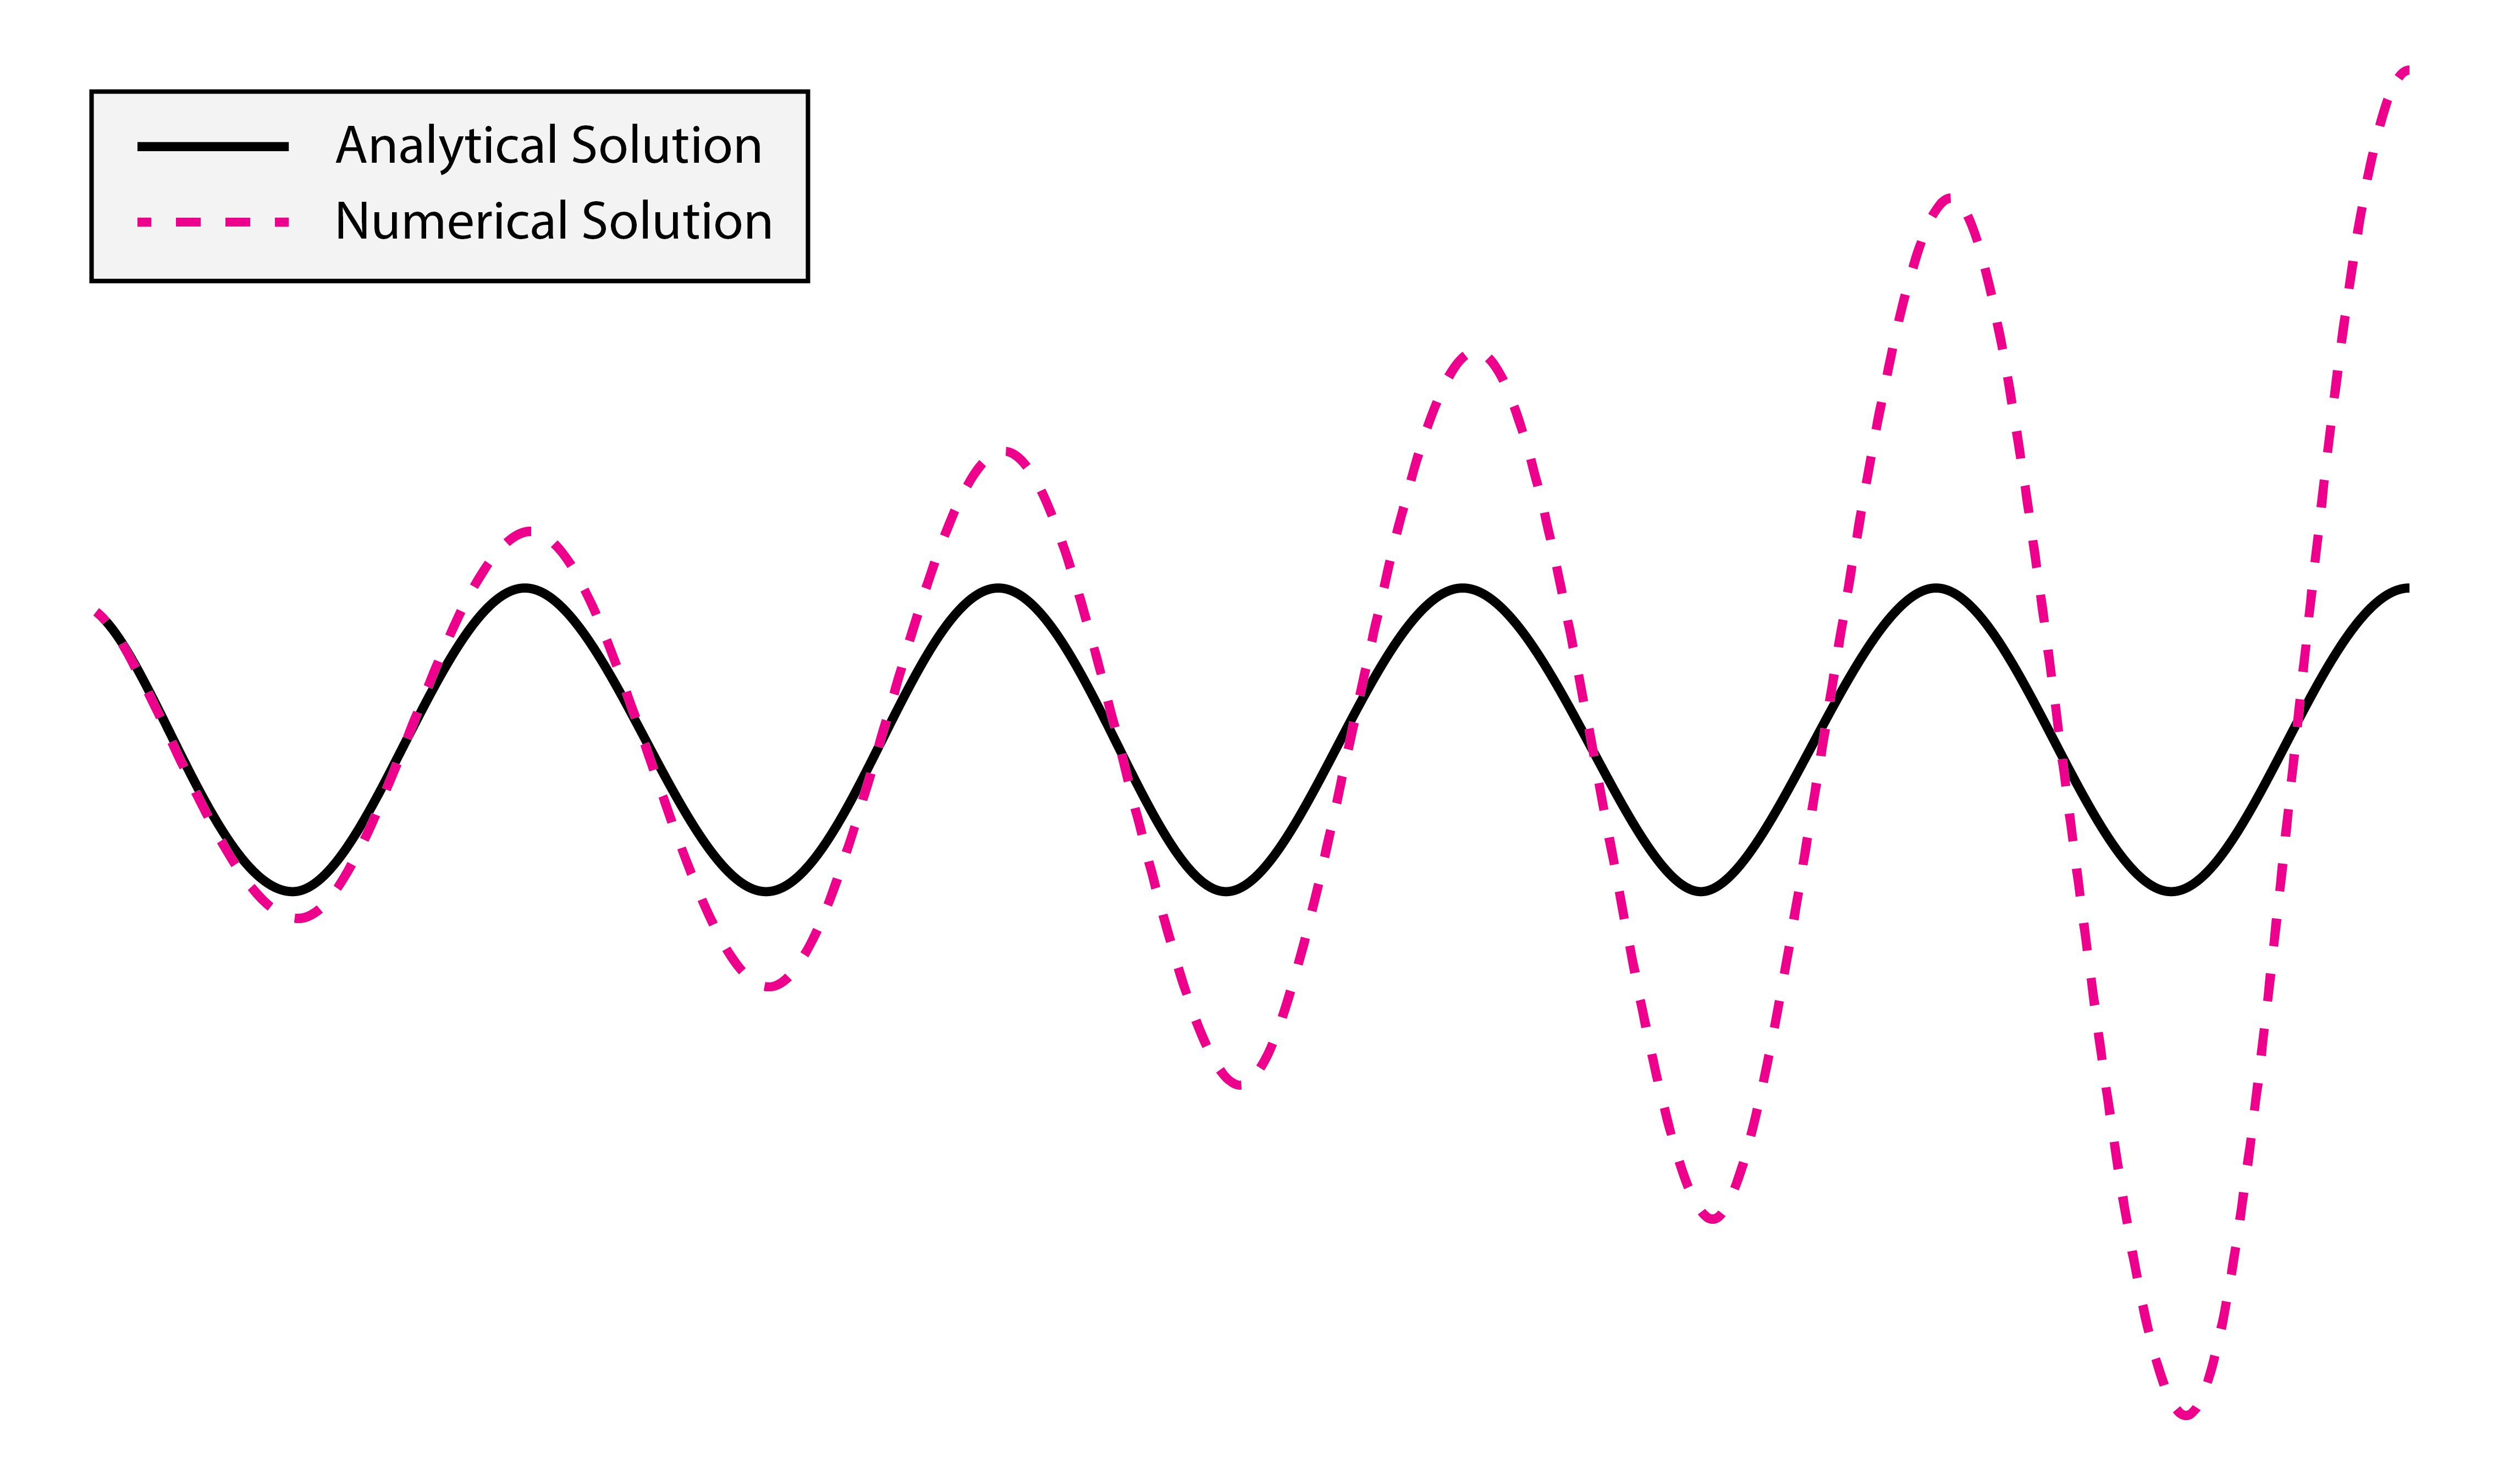
\includegraphics[width=\linewidth]{numericalInstability.png}
  \caption{An example of inaccurate numerical integration causing instability, especially in undamped/underdamped/stiff systems.}
  \label{fig:numericalInstability}
\end{figure}

For linear systems, explicit forward time integration can be achieved using a variety of methods, each with associated error and computational cost.  The simplest and most computationally efficient approach is forward Euler (1\textsuperscript{st} order):
\[ \vec{v}_{t+1} = \vec{v}_{t} +  \vec{a}_{t}\Delta t\]
\[ \vec{p}_{t+1} = \vec{p}_{t} +  \vec{v}_{t}\Delta t\]\\

Verlet integration requires storing the previous two position calculations (at time $t$ and $t-1$) in order to calculate the next position.  The following form of Verlet gives 2\textsuperscript{nd} order position and 1\textsuperscript{st} order velocity calculations:
\[ \vec{p}_{t+1} = 2\vec{p}_{t} - \vec{p}_{t-1} +  \vec{a}_{t}\Delta t^2\]
\[ \vec{v}_{t+1} = \dfrac{\vec{p}_{t+1} - \vec{p}_{t}}{\Delta t}\]\\

Higher order methods such as Runge-Kutta (RK4, 4\textsuperscript{th} order) reduce error further, but require multiple calculations in order to solve for a single time step.  Lower order Runge-Kutta methods, such as the midpoint method, may also be worth exploring.\\

Time integration of rotations is a bit trickier.  The methods described above are meant for intergration in linear space, so they can be applied to the transformation between angular acceleration and velocity.  For example, forward euler of angular acceleration is:
\[ \vec{\omega}_{t+1} = \vec{\omega}_{t} +  \vec{\dot{\omega}}_{t}\Delta t\]

3D rotational space in inherently spherical, and applying linear integration techniques to integrate angular velocity will create large errors when the angular displacement is large.  Instead we can convert angular velocity into quaternion space:
\[ \dot{q} = 1/2\vec{\omega}*q\]
with $\vec{\omega}$ as a 4-space vector with $w=0$ and $*$ denoting the Hamilton product.\\

Euler integration of $\dot{q}$ is as easy as multiplying by $\Delta t$ and normalizing to a unit quaternion:
\[ q = normalize(\dot{q}\Delta t)\]

\subsection{Poisson's Ratio}

\begin{figure}
  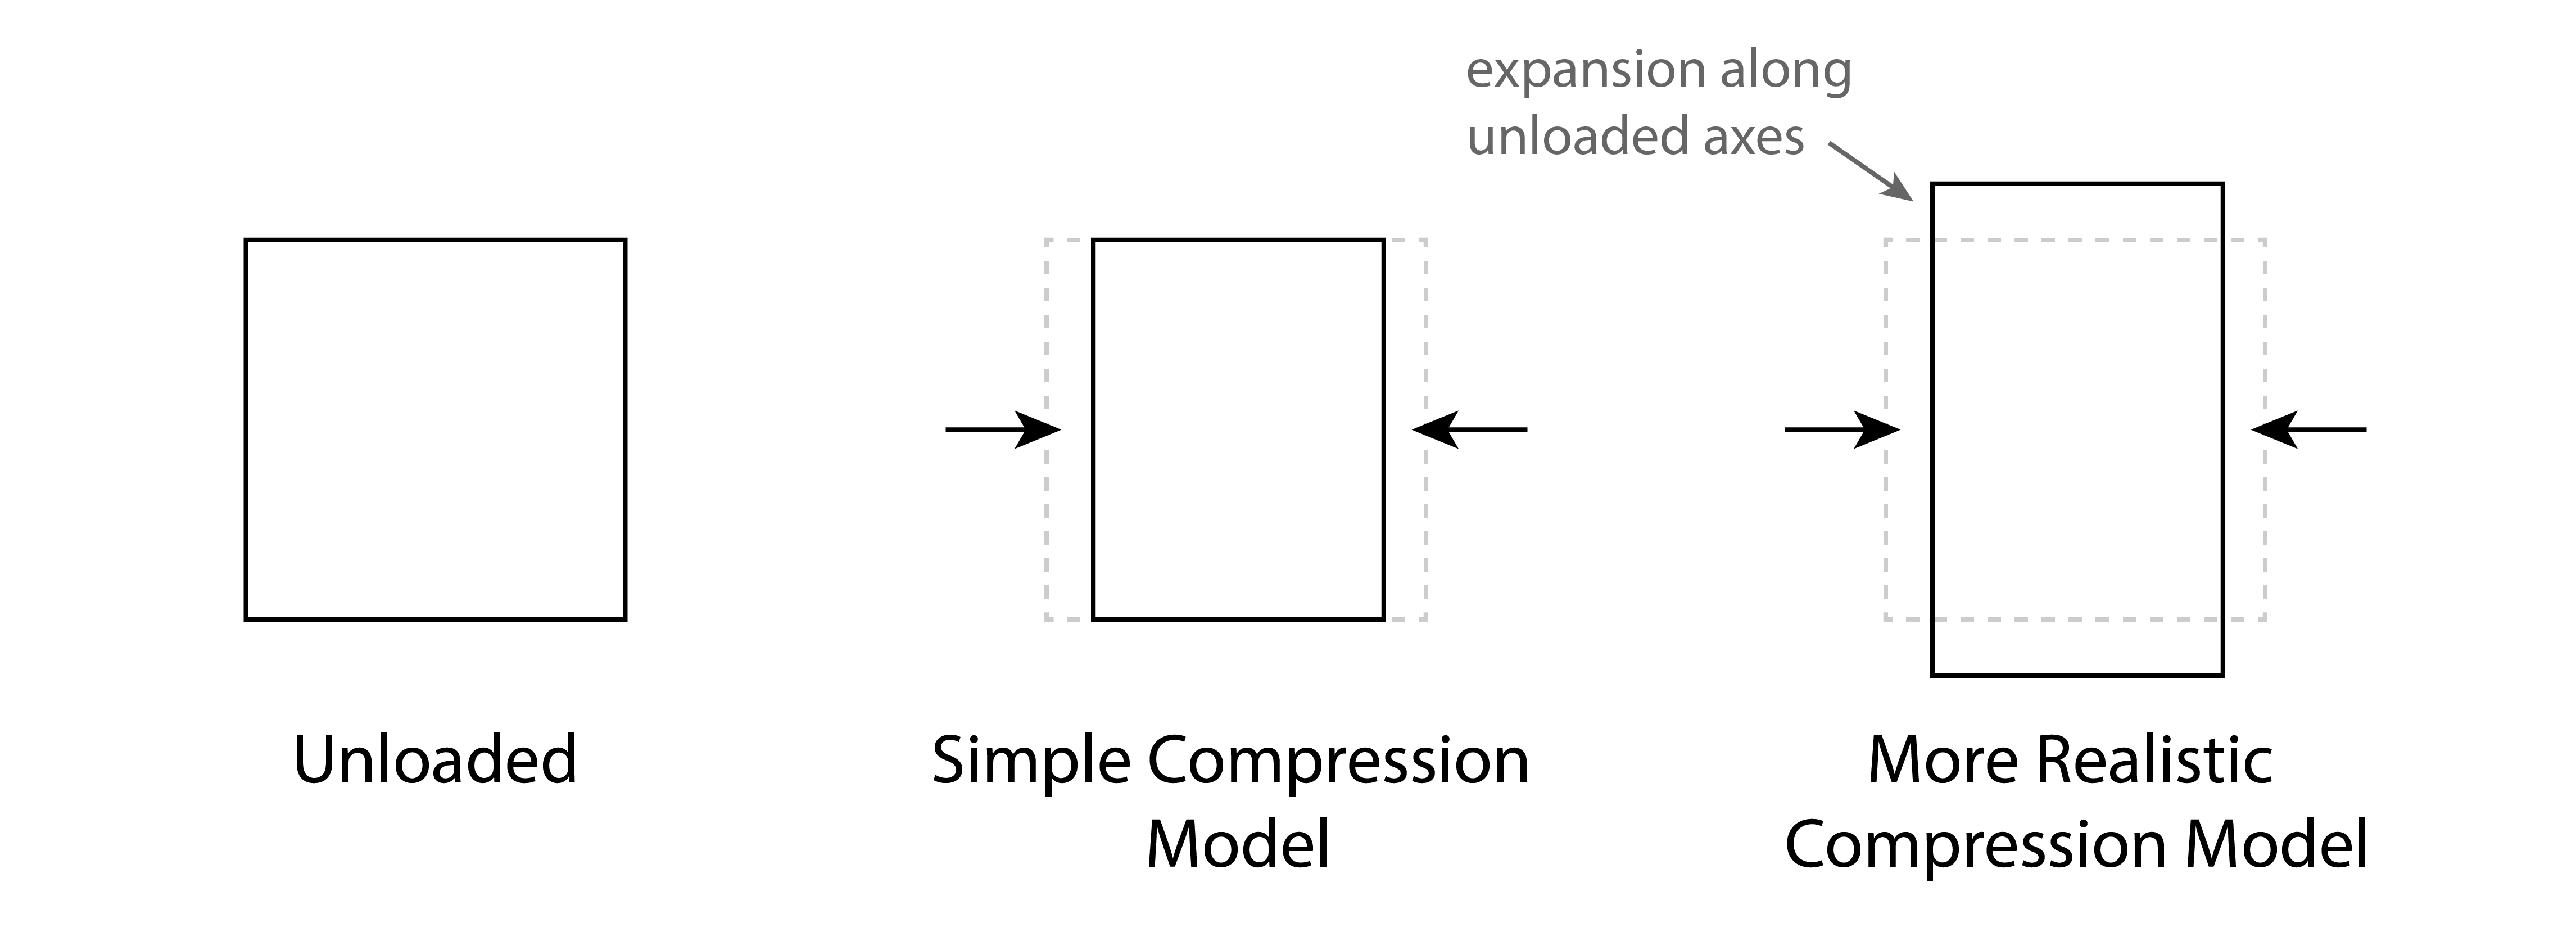
\includegraphics[width=\linewidth]{SolidMechanicsReality.png}
  \caption{Deviation from reality in simple \textit{function} simulation.  Some coupling between degrees of freedom is expected, for example, compression on one axis will result in expansion along other, unloaded axes.}
  \label{fig:SolidMechanicsReality}
\end{figure}

In reality, the degrees of freedom illustrated in Fig \ref{fig:SolidMechanicsDOF} are not completely orthogonal from one another.  For example, compression along one axis of a solid will cause some degree of expansion along the unloaded axes (Fig \ref{fig:SolidMechanicsReality}).  For axial deformations, this effect can be modeled by an additional linear elastic relationship:
\[ \epsilon_{transverse} = -\nu \epsilon_{axial}\]

where $\nu$ is Poisson's ratio and $\epsilon$ are strains in the transverse and axial directions.\\

Though I am not currently modeling this effect in simulation, it could be added in the fullness of time.

%\subsection{Hysteresis}
%
%Hysteresis is a time-dependent effect of the stress/strain curve of a solid.  Typically, solids with internal damping display hysteresis due to conversion of motion to heat.

\subsection{Floating Point Operations}

Finally, the accumulation of error in floating point calculations can potentially throw systems unstable, especially when damping is absent.  In its current JavaScript implementation, floating points numbers are stored as 64 bit in the CPU and 32bit in the GPU.  I'm not currently using any tricks to mitigate floating point error in my code.

\section{Electronic Simulation}\label{sec:electronicSim}

The physics engine currently supports simulation of various types of oscillators (sine, triangle, PWM, and saw) whose frequency, phase, pulse-width, and direction can be adjusted.  Oscillators have two polar outputs, which are connected through wires to actuators.  At each time step, the state of the electronic system is evaluated, and the analog voltage across each actuator is fed into the mechanical simulation.  Errors are thrown when a user incorrectly wires components and renders the electronic simulation unsolvable.\\

In the system we are modeling, electronic effects are orders of magnitude faster than mechanical effects.  Rather simulating the propagation of electronic signals across cells through iterative, local interactions, the state of all electronics is completely solved before each step of mechanical simulation.  This means that it is not currently possible to simulate things like ring oscillators, which rely on a time dependance to be properly modeled.  Depending on the future trajectories of fabrication of electronic components for this system, a time-dependent simulation of electronics may be worth revisiting.

\section{Collision Detection}

Collision detection is needed to simulate interactions with the environment, such as gripping and locomotion.  Simple collision detection with the ground has been implemented using a spring/damper system to model penetration of the ground plane.  Calculation of normal force and friction is also achieved through these interactions.  Currently, the edge of a cell is calculated by the position of its center plus a constant radial offset.  A more accurate model could compute deformations of the cell's mesh using shape functions to determine where its boundaries lie.\\

Care must be taken to avoid inefficient calculation of collisions as it can easily turn into an n-body problem.  The regular structure of the systems we intend to model can be leveraged in computational speedups.  Because everything lies on a regular grid, it is trivial to precompute the cells located on the boundary of a solid object, and only evaluate collisions between these boundary cells.  Additionally, it might be possible to group cells spatially on an octree for collision detection speedups. \\

The goal of collision detection within this thesis is to provide a qualitative assessment of interactions between assemblies and their environment.  Current methods weigh efficiency and simplicity over accuracy.  In its current state, no quantitative conclusions should be drawn from the collision detection.  For example, evaluating this system at different time increments may alter the long term course of the state of the simulation.  Accurate, quantitative modeling of interactions between solids is beyond the scope of this work.

